\documentclass[titlepage]{article}
\usepackage{algpseudocode}
\usepackage{algorithm}
\usepackage{graphicx} % Required for inserting images
\usepackage[utf8]{inputenc}
\usepackage{setspace}
\usepackage{amssymb}
\usepackage{amsmath}
\usepackage{listings}
\usepackage{matlab-prettifier}
\usepackage{url}
\usepackage{hyperref}
\usepackage{float}
\usepackage{caption}
\usepackage{subcaption}
\graphicspath{ {./Images/} }

\title{Sledenje žarku v neevklidskih prostorih}
\author{Blaž Bergant, Martin Jereb, Matjaž Pogačnik}
\date{Matematično modeliranje, maj 2024}

\begin{document}

\maketitle
\newpage
\tableofcontents
\newpage

\section{Uvod}
Algoritem sledenja žarku (\textit{ang. Ray Tracing}) je priljubljen algoritem, uporabljen v 
računalniški grafiki, ki simulira realistično osvetlitev prizorov. Temelji na ideji sledenja 
žarka svetlobe po prizoru, izračunavanju njegovega preseka z objekti in odbijanju v drugo smer. 
Običajno ta algoritem uporabljamo v evklidskem prostoru, saj ta predstavlja resnični svet. 
Vendar pa lahko algoritem implementiramo tudi v drugih (neevklidskih) prostorih, da dobimo 
zanimive vizualne rezultate. To bo glavna naloga tega projekta.

\section{Cilji}
Cilj za projektno nalogo, nam je bil narediti program, v katerem se vsak uporabnik (tudi tak, ki 
ne pozna izvorne kode) lahko vidi razliko med različnimi prostori ki niso evklidski, in 
jih primerja z evklidskim. Želeli smo si, da bi bilo dodajanje novih prostorov in 
novih objektov kar se le da enostavno in da na slike nebi bilo potrebno dolgo čakati.


\section{Sledenje žarkom}
Predstavljajte si, da ste na vaši najljubši plaži, ki ima razgled na ocean. Ko se ozrete na barko,
ki potuje proti sončnemu zahodu, boste poleg tega da se barka oddaljuje opazili tudi, da se "pogreza" 
v tla.

To je ravno zaradi potovanja žarkov. Ker smo v evklidskem prostoru, bo žarek potoval naravnost in nas 
zaradi ukrivljenosti Zemlje po določeni razdalji ne bo več dosegel. Sedaj pa si predstavljajmo, 
da bi lahko barko kljub oddaljevanju še vedno videli celotno. Ta posebna zmožnost bi nam bila 
omogočena v sferičnem neevklidskem prostoru.

\begin{figure}[H]
    \centering
    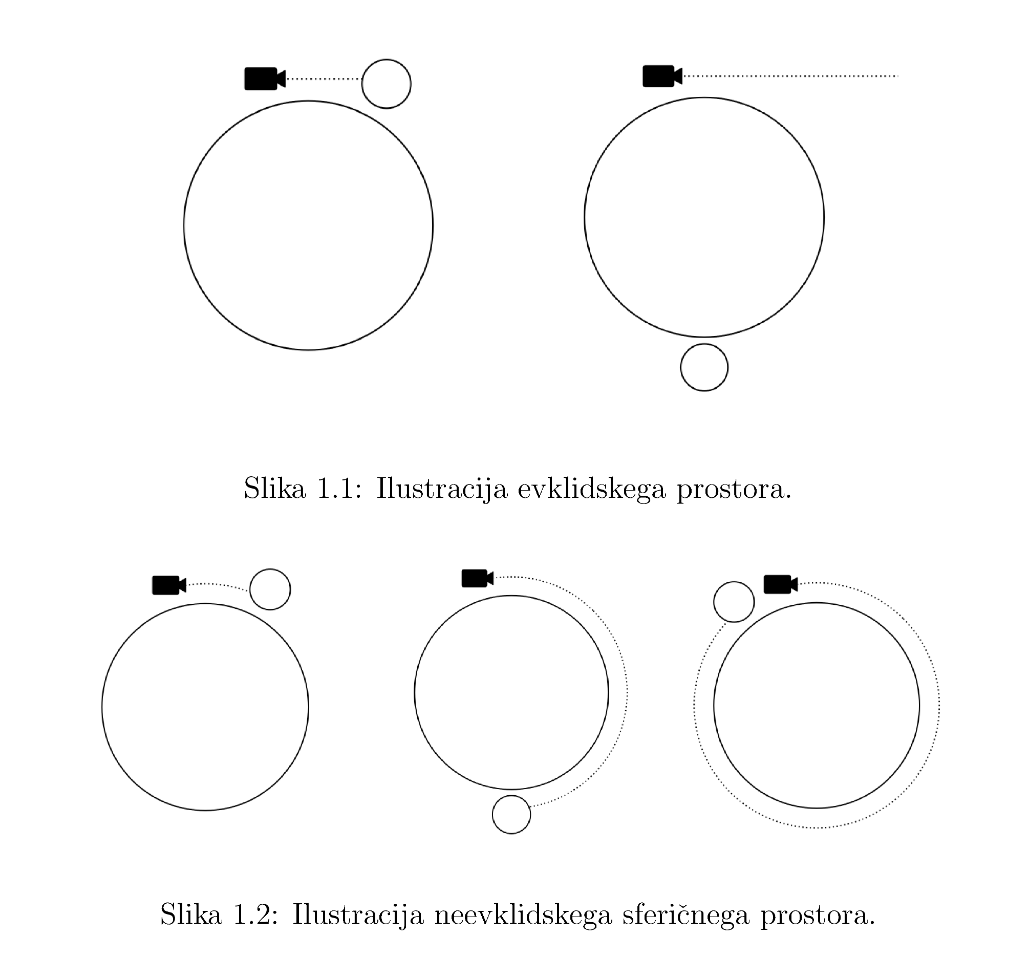
\includegraphics[width=0.5\linewidth]{Images/potovanje_zarkov.png}
    \caption{Primerjava žarka v evklidskem in sferičnem prostoru [Vir: G. Kovač]}
    \label{Slika:Primerjava žarkov evklidski, sferični}
\end{figure}

Kaj pa pravzaprav je neevklidski prostor? To je prostor, ki ne sledi postulatom evklidske geometrije. 
Torej prostor ni raven ampak je ukrivljen, vsota kotov v trikotniku je večja ali pa manjša od 
180 stopinj. Neevklidski prostor delimo na več različnih geometrij med katerimi so 
hiperbolična geometrija, eliptična geometrija, sferična geometrija, projektivna geometrija itd.

\section{Zasnova projekta in osnovni algoritem sledenja žarkov}
Želeli smo si načina podajanja objektov in prostorov, ki bi bil dovolj splošen, da lahko brez
spreminjanja algoritmov dodamo nove.

\subsection{Objekti v sceni}
Posamičen objekt je podan z enačbo, ki sprejme točko v prostoru in vrne vrednost. 
Enačba je torej oblike
\[ o(x,y,z): \mathbb{R}^3 \to \mathbb{R} = a \]
kjer je \(a = 0\) v primeru, da je točka na ploskvi objekta in \( a \neq 0 \) v primeru, da 
je točka v notranjosti ali zunanjosti objekta.
Za kroglo s središčem v $(x_{0}, y_{0}, z_{0})$ in polmerom $r$ je to enačba
\[(x-x_{0})^{2}+(y-y_{0})^{2}+(z-z_{0})^{2}-r^{2}=0, \]
Za ravnino z normalo \( \vec{n} = [a, b, c]^T \) in točko na ravnini $(x_{0}, y_{0}, z_{0})$ pa:
\[ ax+by+cz-(ax_0+by_0+cz_0) = 0. \]

\subsection{Prostori}
Vsak prostor implementira funkcijo v obliki
\[ s_{T, \vec{v}}(t): \mathbb{R} \to \mathbb{R}^3 = [x, y, z]^T \]
ki vrne točko v prostoru, kjer bi bil žarek, ki gre skozi točko \(T\) v smeri \(\vec{v}\), če 
ga premaknemo za razdaljo \(t\) po tem prostoru. Na dvodimenzionalni sferi $\mathbb{S}^{2}$ funkcija računa približek, v primeru evklidskega prostora pa je to preprosto premik po premici za korak \(t\)
\[ \vec{T}_{n+1} = \vec{T}_{n} + t \cdot \vec{v} \]
\bigskip
\newline
Sledenje žarkom na ploščatem torusu in dvodimenzionalni sferi sta podrobneje opisana kasneje.

\subsection{Generiranje žarkov}
Žarek je definiran z začetno točko \(T_{0}\) in enotskim vektorjem \(\vec{v}\). Ker smo si želeli, da 
širino kadra (ang. Field of View) podamo v stopinjah kota, ki ga kamera vidi po diagonali kadra,
smo enotske vektorje \( v \) generirali po postopku:

\begin{enumerate}
  \item Vsi žarki, imajo začetno točko \(T_{0}\) na poziciji kamere
  \item Iz \( FOV \) izračunamo \( FOV_X \) (širino kadra po horizontali), \( FOV_Y \) (širino kadra po vertikali)
  \item Ker so piksli slike štirikotni, lahko zamik v smeri horizontalni in vertikalni smeri izračunamo kot:
  \[\Delta x = \Delta y = \frac{FOV_X}{RES_X} \] kjer je \(RES_X\) širina slike v pikslih.
  \item Žarke predstavimo kot točke na enotski sferi, ki je usmerjena v smer v katero kaže kamera. Vsak žarek, 
  ima azimut \[ \theta = -FOV_X/2 + i \cdot \Delta x \] in elevacijo \[ \phi = FOV_Y/2 - j \cdot \Delta x, \]
  kjer je \( i \) stolpec in \( j \) vrstica slike (šteta po računalničarsko, torej začnemo z 0).
  \item Korektiramo distorcijo žarkov, ki se pojavi, ker sta točki na enotski sferi, ko je \( \phi \) blizu 0 in 
  rotiramo \(\theta =\theta + \Delta x \) veliko bolj oddaljeni, kot ko je \( \phi \) blizu \( \pi/2 \) 
  (kjer bi za vsak \( \theta \) dobili enako točko) \[ \phi_{true} = \phi \cdot cos(\theta) \]
  \item Enotski vektor \( \vec{v} \) dobimo iz azimuta in elevacije kot:
  \[ \vec{v} = [ \cos(\theta) \cos(\phi), \sin(\phi), \cos(\theta) \sin(\phi) ]^T \]
  \item Vektor \(v\) s pomočjo ortogonalnih matrik rotiramo v smer kamere.
\end{enumerate}
Postopek se zdi kar zapleten, vendar je proizvedel bolj natančne rezultate kot druge metode, ko 
kamera ne gleda naravnost, npr. mreža točk za piksle nekoliko pred kamero, kjer za vsak piksel generiramo žarek 
med kamero in točko na mreži. Omogoča nam tudi določanje širine kadra v stopinjah, kar je zelo uporabno.

\begin{figure}[H]
  \centering
  \begin{minipage}[t]{.5\textwidth}
    \centering
    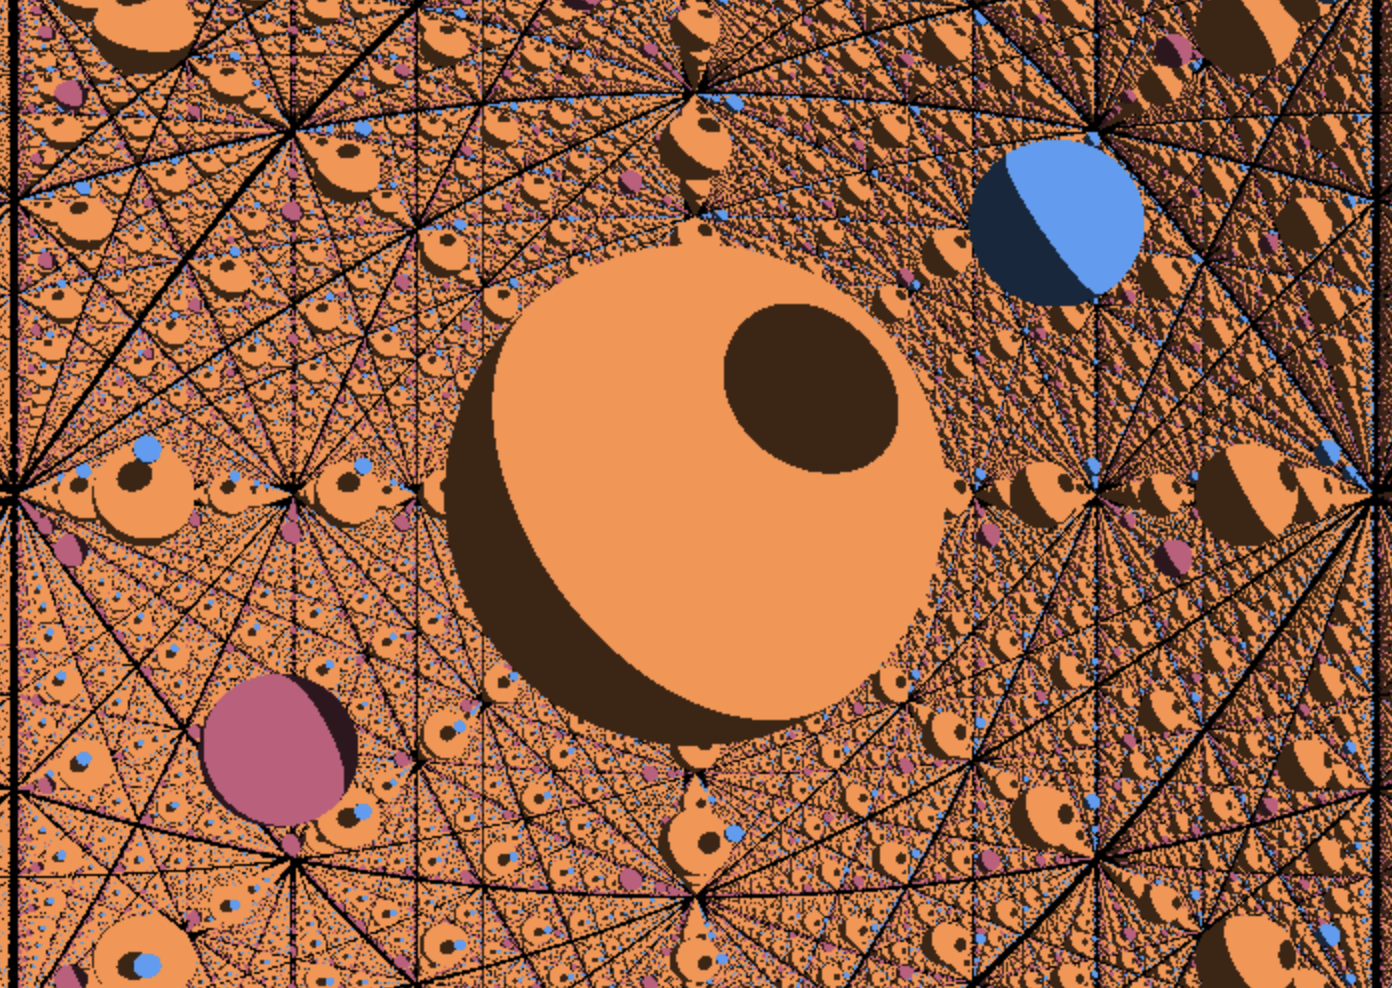
\includegraphics[width=1\linewidth]{Images/Flat_torus_14mm_distorted.png}
    \captionof{figure}{Flat torus z distorzijo}
    \label{fig:Torus distorted}
  \end{minipage}%
  \begin{minipage}[t]{.5\textwidth}
    \centering
    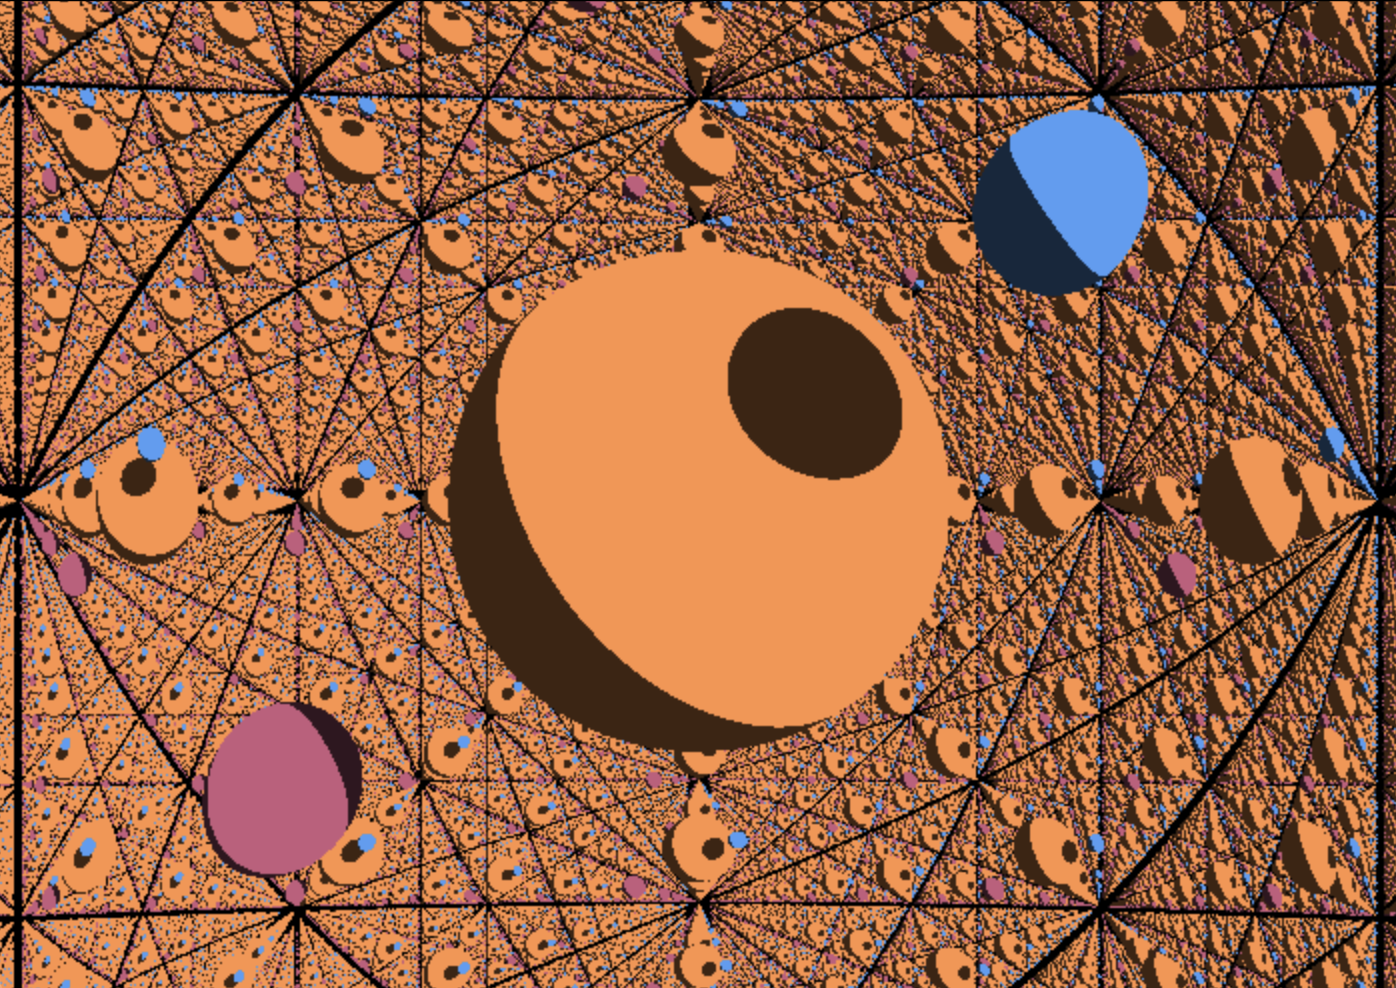
\includegraphics[width=1\linewidth]{Images/Flat_torus_14mm_undistorted.png}
    \captionof{figure}{Flat torus brez distorzije}
    \label{fig:Torus undistorted}
  \end{minipage}
  \end{figure}

Zgoraj je primerjava slike prostora flat torus, kjer je širina kadra ekvivalentna 14mm objektivu. Na levi je 
prikazana slika, ki ne upošteva popravka za distorzijo (korak 5), na desni pa je slika, ki ga upošteva.

Opazimo lahko, da so horizontalne črte na desni sliki dejansko horizontalne, medtem ko so na levi sliki 
ukrivljene. Ker je kader usmerjen za 10 stopinj navzgor, se vertikalne črte na robovih ukrivijo navznoter, 
kar je pojav, ki se zgodi tudi na pravih kamerah.


\subsection{Sledenje žarkom}
Osnovni algoritem sledenja žarkov je sledeč:

\begin{enumerate}
\item V poljubnem prostoru premikamo žarek s pomočjo enačbe \( s(t) = [x, y, z]^T \) za korak velikosti $h$.
\item Za vsak objekt, s pomočjo njegove enačbe \( o(x, y, z) = a \) preverimo, če je žarek prešel skozi ploskev 
objekta (če je \( a \) spremenil predznak).
\item Če je za nek objekt \( a \) spremenil predznak, razpolovimo korak \( h = h/2 \) in ponovimo korak.
\item Postopek razpolavljanja ponavljamo, dokler korak ni manjši od \( \varepsilon \).
\end{enumerate}

\begin{figure}[H]
  \centering
  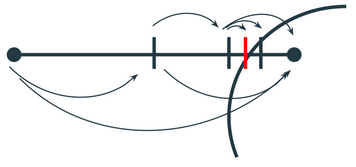
\includegraphics[width=0.5\linewidth]{intersect.png}
  \caption{Iskanje natančnejšega presečišča}
  \label{Slika:Iskanje natančnejšega presečišča}
\end{figure}

\subsection{Računanje barve piksla}
Vsak žarek obarvamo z barvo objekta s katerim se je sekal, oziroma črno, če se ni z nobenim. Za senčenje moramo
poslati še en žarek od presečišča proti luči. 
\begin{enumerate}
  \item Poiščemo vektor, ki gre v smeri od presečišča do luči: 
  \[ \vec{v} = \frac{\vec{r}_{l} - \vec{r}_{p}}{||\vec{r}_{l} - \vec{r}_{p}||} \]
  Kjer je \( \vec{r}_{l} \) krajevni vektor luči, \( \vec{r}_{p} \) pa krajevni vektor presečišča.
\item Če žarek, ki se začne v točki presečišča in gre v smeri \( \vec{v} \), seka kakšen objekt preden 
    prepotuje razdaljo do luči 
  \( d = ||\vec{r}_{l} - \vec{r}_{p}||\), potem je presečišče v senci.
\end{enumerate}


\section{Evklidski prostor in potovanje žarka do luči}

V evklidskem prostoru je potovanje žarkov preprosto premik po premici: 
\[ \vec{T}_{n+1} = \vec{T}_{n} + t \cdot \vec{v} \]
Žarki potujejo naravnost, kot smo navajeni. Algoritem sledenja žarkov je enak 
kot v primeru ploščatega torusa, le da žarkov ni potrebno preslikati. 

Odločili smo se, da bodo žarki od presečišča z objektom do luči potovali kar po evklidskem prostoru. 
To odločitev smo sprejeli, ker bi bilo v neevklidskih prostorih zelo težko implementirati algoritem, 
ki žarek pošlje po vseh poteh, ki vodijo do vsaj ene luči. Zadovoljiti bi se morali z algoritmom,
ki žarke pošilja v razne smeri in upa, da bo vsaj en žarek prišel do luči, če pot do nje obstaja. 
Implementacija tega predstavlja izboljšavo, ki bi jo lahko dodali v prihodnosti.

\begin{figure}[H]
  \centering
  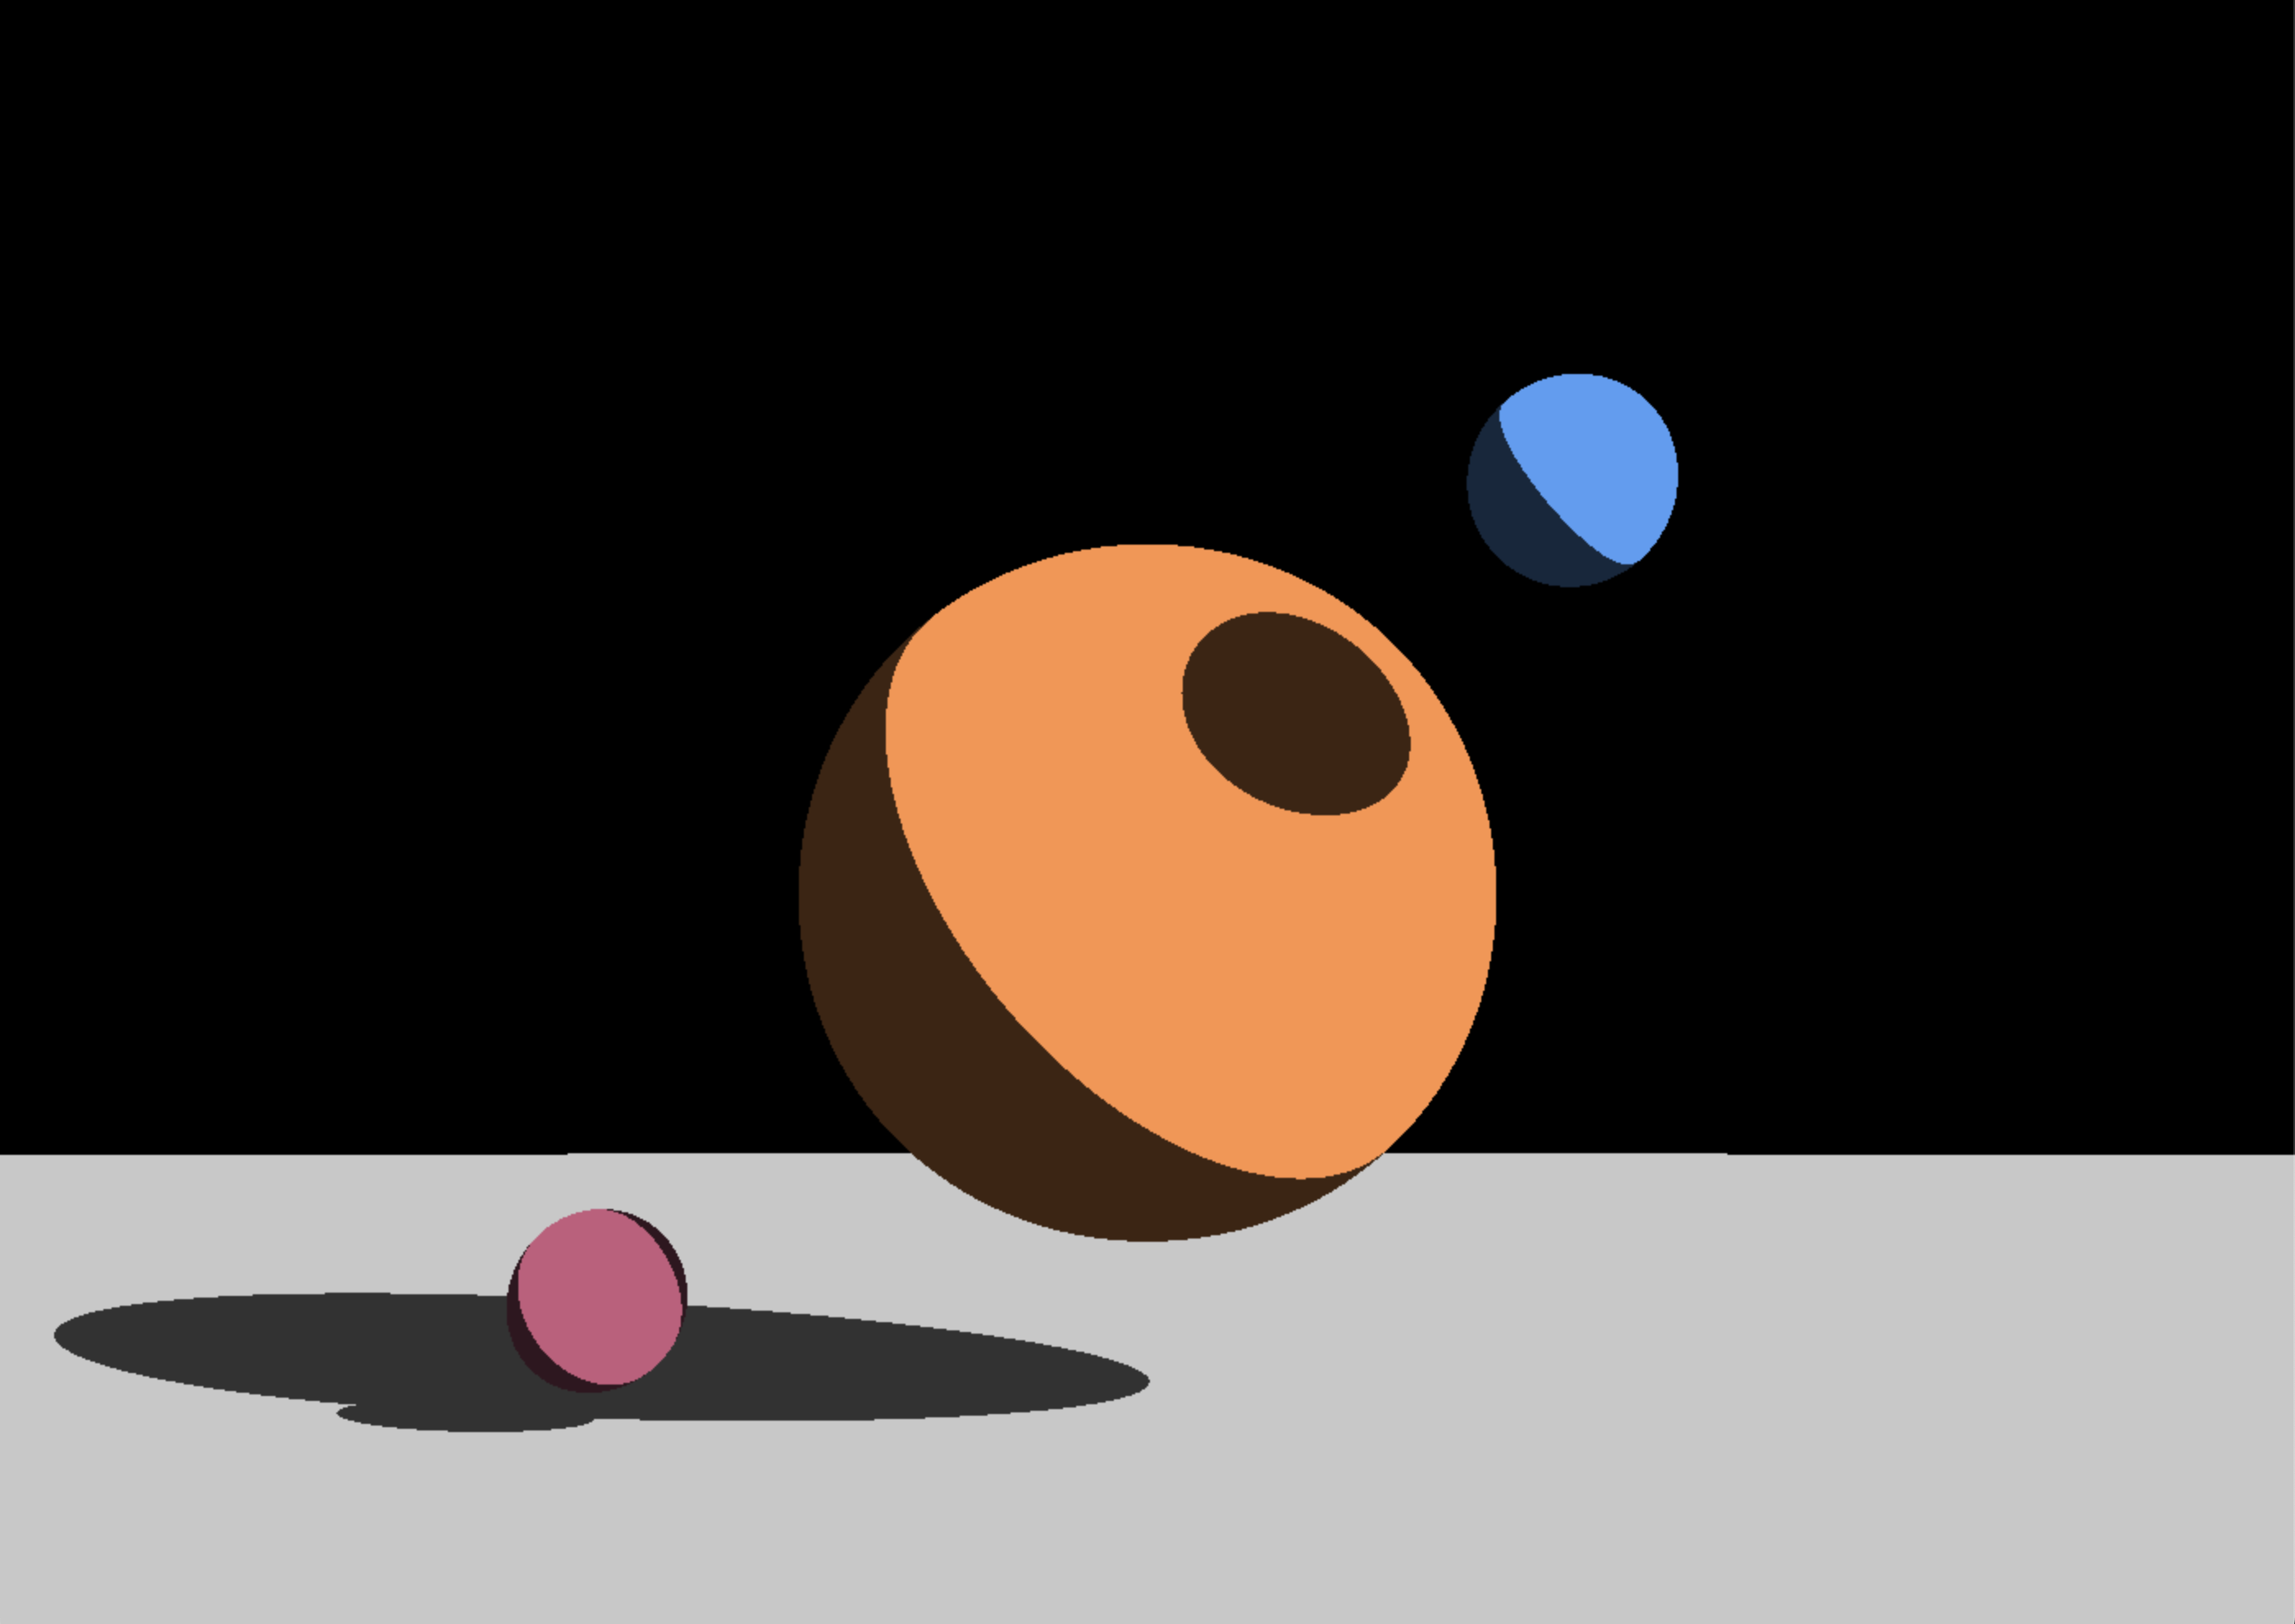
\includegraphics[width=0.8\linewidth]{Images/Euclidean_24mm.png}
  \caption{Evklidski prostor}
  \label{Slika:Euklidski prostor}
\end{figure}

Na sceni kamera gleda v krogle obrnjena za 10 stopinj navzgor. Enaka scena 
bo uprizorjena tudi v drugih prostorih.

\section{\texorpdfstring{Sledenje žarkom na ploščatem torusu \( \mathbb{T}_{pl}^{3} \)}{Sledenje žarkom na flat torusu}}

\subsection{Kaj je tri dimenzionalni ploščat torus \( \mathbb{T}_{pl}^{3} \) ?}
Tri dimenzionalni flat torus \( \mathbb{T}^3_{pl} \) je prostor, ki ga dobimo tako, da združimo nasprotne ploskve enotske kocke \([0,1] \times [0,1] \times [0,1] \subset \mathbb{R}^3 \), kjer je \(\mathbb{R}^3\) tridimenzionalni evklidski prostor. Formalno pravimo, da je \( \mathbb{T}^3_{pl} \) kvocient \(\mathbb{R}^3\) z grupo translacij:
\[
(x, y, z) \to (x \pm 1, y, z), \quad (x, y, z) \to (x, y \pm 1, z), \quad (x, y, z) \to (x, y, z \pm 1).
\]

Običajni torusi so ukrivljeni in se jim ukrivljenost po površini spreminja. Flat torus pa ima konstantno ukrivljenost v vsaki točki. Poimenovanje flat izhaja iz tega, ker je povsod podoben navadni evklidski ravnini. Podobno velja za tridimenzionalni flat torus, kjer pri sledenju žarka lahko uporabimo kar osnovno definicijo žarka. Ključna razlika med algoritmom v \( \mathbb{R}^3 \) in \( \mathbb{T}^3_{pl} \) pa je, da bomo tokrat dodali še en korak, ker moramo žarek omejiti na kocko. Dokler se nahajamo znotraj njenih meja, ne naredimo nobenih popravkov. Ko pa ugotovimo presečišče z eno od ploskev, moramo žarek preslikati na nasprotno ploskev. To lahko storimo tako, da preprosto žarek omejimo znotraj domene, izračunamo presežek in ga prištejemo začetku domene.

\begin{figure}[H]
    \centering
    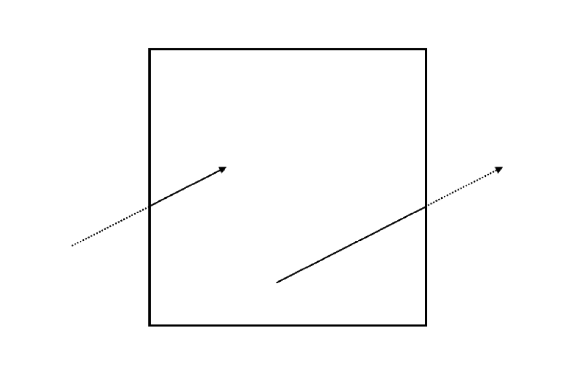
\includegraphics[width=0.5\linewidth]{Images/flat_torus_zrcaljenje.png}
    \caption{Žarek v dvodimenzionalnem flat torusu}
    \label{Slika:Žarek v dvodimenzionalnem flat torusu}
\end{figure}
\subsection{Algoritmi za flat torus}
Ključna sprememba v primerjavi z običajnim prostorom $\mathbb{R}^{3}$ je ta, da žarek omejimo na kocko $[a,b]^{3}$. V spodnji funkciji mapToCube je $T_{n}$ začetni vektor, a in b pa meje intervala $[a,b]$.
\begin{algorithm}[H]
\caption{Map to Cube}\label{alg:mapToCube}
\begin{algorithmic}[1]
\Function{mapToCube}{$T_{n}$, $a$, $b$} 
    \State $range \gets b - a$
    \State $q \gets (T_{n} - a) / range$
    \State $fraction \gets q - \text{floor}(q)$
    \State $T_{n+1} \gets a + fraction \cdot range$
    \State \Return $T_{n+1}$
\EndFunction
\end{algorithmic}
\end{algorithm}

Funkcija \textbf{traceRayFlatTorus} sprejme začetno točko $T_{0}$, smer $\vec{v}$, korak step, maksimalno število iteracij maxIt, množico objektov objects in meje $a$ in $b$.
Pomožni funkciji \textbf{signs} in \textbf{checkIntersect} implementirata funkcije objektov \( o(x,y,z) \).
\begin{algorithm}[H]
    \caption{Sledenje žarku na flat torusu}
\begin{algorithmic}
    \Function{traceRayFlatTorus}{$T_{0}$, $\vec{v}$, step, maxIt, objects, a, b, $\varepsilon$}

    \State $T_{n}$, $T_{n+1}$ $\gets$ $T_{0}$
    \State signs $\gets$ \textbf{signs}($T_{n}$, objects)
    \Comment{izračunamo začetne predznake}
    \\
    \State t $\gets$ 0
  \While{true}
    \If{t == maxIt}
      \State \Return{-1}
    \ElsIf{step $<$ $\varepsilon$}
      \State \Return{$T_{n}$}
    \EndIf
    \State $T_{n+1}$ $\gets$ $T_{n}+step \cdot \vec{v}$
    \State $T_{n+1}$ $\gets$ \textbf{remap}($T_{n+1}$, a, b)
    \\
    \Comment{naredimo korak, preslikamo na željeno domeno}
    \\
    \State signs $\gets$ \textbf{checkIntersects}($T_{n+1}$, objects, signs)
    \\
    \Comment{preverimo, če smo sekali objekt}
    \\
    \Comment{če da, razpolovimo korak}

    \If{object != NULL}
        \State step $\gets$ step/2
    \Else
      \State $T_{n}$ $\gets$ $T_{n+1}$
      \State t $\gets$ t+1
    \EndIf
  \EndWhile
\EndFunction
\end{algorithmic}
\end{algorithm}

\newpage
\subsection{Interpretacija rezultatov}
Ko program poženemo, dobimo lep vizualni rezultat.
\begin{figure}[H]
    \centering
    \includegraphics[width=0.7\linewidth]{Images/flat_torus_24mm_500.png}
    \caption{Rezultat "ray tracinga" za tri dimenzionalni flat torus (500 preslikanj), kjer scena nima ravnine.}
    \label{Slika:Rezultat "ray tracinga" za tri dimenzionalni flat torus}
\end{figure}
Na sliki lahko opazimo podoben efekt tistemu v hišah iluzij, ko smo v sobi polni ogledal. Razlika je v tem, 
da se tu žarki ne odbijejo, temveč "teleportirajo" na drugo stran scene, zato slika ni simetrična. Na levi strani slike 
lahko opazujemo sceno, kot bi izgledala, če bi jo gledali bolj z desne strani, na desni pa kot da bi jo gledali z leve.

Izrišejo se tudi distinktne črte. Nekateri žarki, ki so kljub velikemu številu preslikavanj
(v tem primeru 500) še vseeno črni, se ne bodo nikoli srečali z objektom, ker gredo v smer, ki je povsem vzporedna
z objekti v "sosednjih" scenah.

\section{\texorpdfstring{Sledenje žarkom na dvodimenzionalni sferi \( \mathbb{S}^2 \)}{Sledenje žarkom na dvodimenzionalni sferi}}
Žarek na dvodimenzionalni sferi bo potoval po najravnejši poti, tj. geodetki, kjer je majhen korak v \( uv \) ravnini opisan s sistemom dveh diferencialnih enačb drugega reda.
\begin{equation}
    \begin{split}
        &\frac{d^{2}u}{dt^{2}}-\cos(u)\sin(u)\frac{dv}{dt}\frac{dv}{dt}=0 \\
        &\frac{d^{2}v}{dt^{2}}+2\cot(u)\frac{du}{dt}\frac{dv}{dt}=0
    \end{split}
\end{equation}

Po krivulji se bomo v nadaljnjih algorimih premikali s pomočjo aproksimacijskih metod, zato moramo sistem DE drugega reda preoblikovati v
sistem DE prvega reda. Za to uvedemo 4 nove spremenljivke
\begin{equation}
\begin{split}
    &y_{1}=u, \quad y_{2}=\frac{dy_{1}}{dt}, \\
    &y_{3}=v, \quad y_{4}=\frac{dy_{3}}{dt}
\end{split}
\end{equation}
Dobimo sistem 4 DE prvega reda
\begin{equation} \label{e:geoSys}
\begin{split}
    &\frac{dy_{1}}{dt}=y_{2} \\
    &\frac{dy_{2}}{dt}=\cos(y_{1})\sin(y_{1})y^{2}_{4} \\
    &\frac{dy_{3}}{dt}=y_{4} \\
    &\frac{dy_{4}}{dt}=-2\cot(y_{1})y_{2}y_{4}
\end{split}
\end{equation}
Ker se bomo premikali po \( uv \) ravnini, moramo koordinate v kartezičnem koordinatnem sistemu transformirati v parametra \( u \) in \( v \). Sfera v \(\mathbb{R}^3\) je
parametrizirana kot
\begin{equation} \label{e:toXYZ}
    \begin{split}
        &X=R\cos(v)\sin(u) \\
        &Y=R\sin(v)\sin(u) \\
        &Z=R\cos(u)
    \end{split}
\end{equation}
\( u \) lahko dobimo kot
\begin{equation} \label{e:toU}
        u=\cos^{-1} \left( \frac{Z}{R} \right)
\end{equation}
za \( v \) pa uporabimo prvi dve enačbi
\begin{equation} \label{e:toV}
    \begin{split}
        &\frac{R\sin(u)Y}{R\sin(u)X}=\frac{\sin(v)}{\cos(v)} \\
        &v=\tan^{-1} \left(\frac{Y}{X} \right)
    \end{split}
\end{equation}
\newpage
Za sledenje žarku po geodetki, si moramo poleg začetne točke izbrati še začetno smer
\(\left( \frac{du}{dt}, \frac{dv}{dt} \right) \). Tako kot pri ostalih prostorih v nalogi, 
bomo uporabili perspektivno projekcijo, kar pomeni da vsi žarki izvirajo iz ene točke in 
niso paroma vzporedni. Od tu dalje imamo svobodo pri izbiri sfer, po katerih bodo žarki potovali. V tej nalogi smo za
vsak žarek izračunali središče sfere z najnižjo \( z \) koordinato in polmerom \( R \). Žarki bodo vedno "zavijali" navzdol, torej se bodo premikali po poldnevnikih.

\begin{figure}[H]
\centering
\begin{minipage}{.5\textwidth}
  \centering
  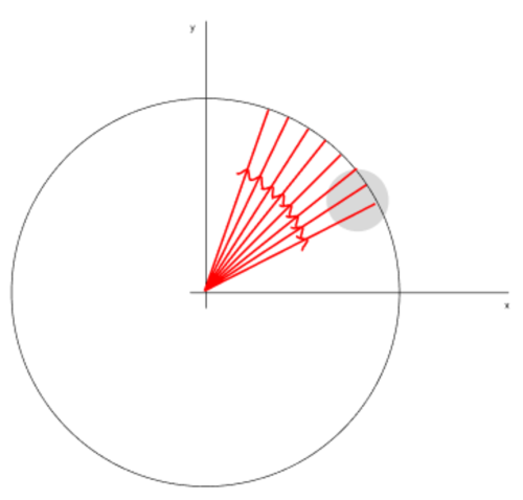
\includegraphics[width=0.8\linewidth]{Images/rays_top.png}
  \captionof{figure}{Potovanje žarkov od zgoraj}
  \label{fig:test1}
\end{minipage}%
\begin{minipage}{.5\textwidth}
  \centering
  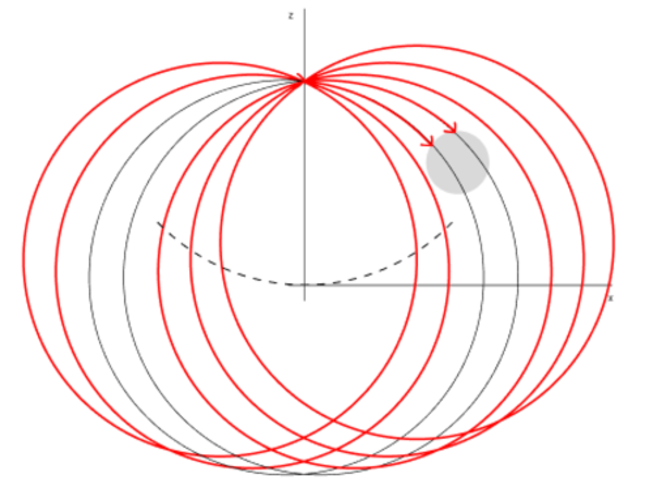
\includegraphics[height=0.77\linewidth]{Images/rays_side.png}
  \captionof{figure}{Potovanje žarkov s strani}
  \label{fig:test2}
\end{minipage}
\end{figure}
\bigskip
\newline
Za različne smeri žarkov \(\vec{v}_{i} \) je bilo središče \( C_{i} \) izračunano po sledečem postopku:
\bigskip
\newline
Izračunamo vektorski produkt med navpičnim vektorjem in smerjo \( \vec{v}_{i} \). Dobljeni vektor je normala na ravnino krožnice z iskanim središčem, ki gre skozi \( T_{0} \)
\begin{equation} \label{e:sphC1}
    \vec{n}_{i}=(0, 0, -1) \times \vec{v}_{i}
\end{equation}
Vektor, ki od \( T_{0} \) kaže proti iskanemu središču, bo ležal v tej ravnini, poleg tega pa bo pravokoten na \( \vec{v}_{i} \). Ponovno uporabimo vektorski
produkt
\begin{equation}\label{e:sphC2}
    \vec{c}_{i}= \vec{v}_{i} \times \vec{n}_{i}
\end{equation}
Krajevni vektor središča nato dobimo tako, da se premaknemo za polmer \( R \) v smeri \( \vec{c}_{i} \)
\begin{equation}\label{e:sphC3}
    \vec{r}_{ci}=\frac{\vec{c}_{i}}{\left \| \vec{c}_{i}\right \|} \cdot R + T_{0}
\end{equation}

\begin{figure}[H]
    \centering
    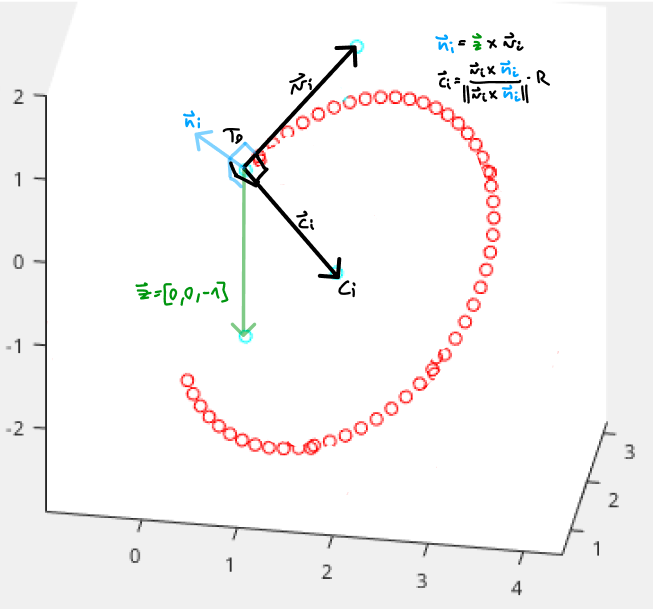
\includegraphics[width=0.8\linewidth]{Images/sredisca.png}
    \caption{Postopek računanja središč krožnic}
    \label{fig:centers}
\end{figure}

Za korak po geodetki bomo \( T_{0} \) najprej premaknili za vektor \( \vec{r}_{ci} \), tako da bo središče sfere v koordinatnem izhodišču. Nato naredimo
korak, novo točko \( T_{i1} \) pa premaknemo nazaj za vektor \( \vec{r}_{ci} \).
Ker želimo potovati po poldnevnikih, bomo za začetno smer \(\left( \frac{du}{dt}, \frac{dv}{dt} \right) \) izbrali \(\left( \pm1, 0 \right) \). Korak po poldnevniku bo v \( xy \) ravnini tako že pravilno obrnjen, določiti pa moramo predznak premika po \( u \) glede na to, ali se premikamo v pravo smer \( \vec{v}_{i} \). To preverimo s skalarnim produktom:
\bigskip
\newline
Naredimo korak v smeri \(\left( 1, 0 \right) \) in označimo dobljeno točko s \( T_{t} \). Vektor v smeri od \( T_{0} \) do \( T_{t} \) označimo z \( \vec{v}_{t} \).
Izračunamo skalarni produkt
\begin{equation} \label{e:dirCorr}
    a= \vec{v}_{i} \vec{v}_{t}^T
\end{equation}
Če se premikamo v pravi smeri, bo \( a > 0 \), drugače moramo za začetno smer izbrati negativni predznak.
\bigskip
\newline
V nadaljevanju se premikamo po geodetki z eno izmed aproksimacijskih metod. V splošnem lahko za take sisteme uporabimo Eulerjevo metodo
\begin{equation} \label{e:euler}
    \begin{split}
        &t_{n+1}=t_{n}+h \\
        &\vec{y}_{n+1}=\vec{y}_{n}+h \cdot \vec{f}(t_{n}, \vec{y}_{n})
    \end{split}
\end{equation}
problem pa se pojavi pri \( \cot(y_{1}) \) v eni izmed enačb, ki ima pole pri
\( k\pi \), \( k \in \mathbb{Z} \). Da se temu izognemo, ne smemo uporabljati fiksne dolžine koraka, temveč moramo uporabiti adaptivne metode, kot je DOPRI5,
ki z uporabo večih metod estimira napako približka in temu primerno prilagodi korak.
\bigskip
\newline
Algoritmi, ki implementirajo opisane metode so predstavljeni v naslednjem poglavju.
\newpage

\subsection{Algoritmi za 2-sphere}
Funkcija \textbf{traceRay2Sphere} sprejme začetko točko $T_{0}$, smer $\vec{v}$, velikost koraka step, maksimalno število iteracij maxIt, množico objektov objects, polmer sfere $\mathbb{S}^2$ in natančnost presečišča $\varepsilon$. 
Pomožna funkcija \textbf{sphereCenter} implementira formule \eqref{e:sphC1}, \eqref{e:sphC2}, \eqref{e:sphC3}, \textbf{initializeSphere} formule \eqref{e:geoSys}, \eqref{e:toU}, \eqref{e:toV}, \textbf{uvToVec} pa formulo \eqref{e:toXYZ}. Funkcija \textbf{DOPRI5} predstavlja implementacijo DOPRI5, ki naredi po en korak glede na trenutno velikost koraka, in skupaj s približkom vrne tudi novo velikost koraka. Tu lahko uporabimo tudi katero drugo adaptivno funkcijo. Ostale funkcije so opisane v
razdelku 
\begin{algorithm}
    \caption{Sledenje žarku na sferi \(\mathbb{S}^{2}\)}
\begin{algorithmic}
    \Function{traceRay2Sphere}{$T_{0}$, $\vec{v}$, step, maxIt, objects, R, $\varepsilon$}

    \State $T_{n}$, $T_{n+1}$ $\gets$ $T_{0}$
    \State signs $\gets$ \textbf{signs}($T_{n}$, objects)
    \Comment{izračunamo začetne predznake}
    \State center, I
    \\
    \State t $\gets$ 0
  \While{true}
    \If{t == maxIt}
    \State \Return{-1}
    \ElsIf{step == 0}
      \State center $\gets$ \textbf{sphereCenter}($T_{0}$, d, R)
      \\
      \Comment{žarku poiščemo središče sfere}
      \State $T_{m}$ $\gets$ $T_{0} - \hbox{center}$
      \Comment{sfero premaknemo v $(0, 0)$}
      \State $\vec{y}_{n}$ $\gets$ \textbf{initializeSphere}($T_{0}$, R)
      \Comment{pripravimo začetni $\vec{y}$}
    \EndIf
    \\
    \State $\vec{y}_{n+1}, \hbox{step}$ $\gets$ \textbf{DOPRI5}($\vec{y}_{n}$, step)
    \Comment{korak po geodetki}
    \State $T_{n+1}$ $\gets$ \textbf{uvToVec}($\vec{y}_{n+1}$, R) + center
    \\
    \State object $\gets$ \textbf{checkIntersects}($T_{n+1}$, objects, signs)
    \\
    \Comment{preverimo, če smo sekali objekt}
    \\
    \Comment{če da, poiščemo natančno presečišče}

    \If{object != NULL}
      \State I $\gets$ \textbf{findIntersection}($T_{n}$, object, signs, $\vec{y}_{n}$, step, R, center, $\varepsilon$)
      \State \Return{I}
    \Else
      \State $\vec{y}_{n}$ $\gets$ $\vec{y}_{n+1}$
      \State $T_{n}$ $\gets$ $T_{n+1}$
      \State t $\gets$ t+1
    \EndIf
  \EndWhile
\EndFunction
\end{algorithmic}
\end{algorithm}

\begin{algorithm}[H]
    \caption{Iskanje natančnejšega presečišča}
\begin{algorithmic}
    \Function{findIntersection}{$T_{0}$, object, signs, $\vec{y}_{n}$, step, R, center, $\varepsilon$}

    \State $T_{n}$, $T_{n+1}$ $\gets$ $T_{0}$
    \\
  \While{true}
    \If{step $<$ $\varepsilon$}
      \State \Return{$T_{n}$}
    \EndIf
    \State $\vec{y}_{n+1}, \hbox{step}$ $\gets$ \textbf{euler}($\vec{y}_{n}$, step)
    \State $T_{n+1}$ $\gets$ \textbf{uvToVec}($\vec{y}_{n+1}$, R) + center
    \\
    \Comment{korak po geodetki z Eulerjevo metodo}
    \State object $\gets$ \textbf{checkIntersects}($T_{n+1}$, object, signs)
    \\
    \Comment{preverimo, če smo sekali objekt}
    \\
    \Comment{če da, razpolovimo korak}

    \If{object != NULL}
        \State step $\gets$ step/2
    \Else
      \State $\vec{y}_{n}$ $\gets$ $\vec{y}_{n+1}$
      \State $T_{n}$ $\gets$ $T_{n+1}$
    \EndIf
  \EndWhile
\EndFunction
\end{algorithmic}
\end{algorithm}

\newpage
\subsection{Interpretacija rezultatov}
Za prikaz značilnosti slik generiranih na dvodimenzionalni sferi $\mathbb{S}^{2}$ smo generirali sliko scene z dvema različno velikima kroglama, kjer je 
vir svetlobe "skrit" za eno izmed krogel. Na \hyperref[fig:2sphRays]{sliki žarkov} vidimo dva snopa žarkov z zaporednimi rdečimi točkami, ki predstavljajo korake. Podobno so z modrimi točkami prikazani žarki proti viru svetlobe. Na \hyperref[fig:2sphRend]{generirani sliki} so piksli, katerim pripadata snopa žarkov, označeni z rdečo. Opazujemo moder objekt na generirani sliki, ki mu pripada manjša izmed krogel, ki se na generirani sliki pojavi v dveh delih, kjer je en delno osvetljen. Rezultat je pričakovan, saj bodo do neke meje zgornji žarki zaokrožili do krogle in jo tako zadeli iz spodnje strani. Ta stran je tudi edina, ki je delno osvetljena, kar lahko vidimo iz uspešne nadaljnje poti žarkov proti viru svetlobe. Ko se premikamo nižje po stolpcu bodo žarki obhajali kroglo, dokler ne bomo dovolj nizko, da jo spet direktno zadanemo. Tokrat žarki ne bodo uspeli priti do vira svetlobe.
\begin{figure}[H]
\centering
\begin{minipage}{.5\textwidth}
  \centering
  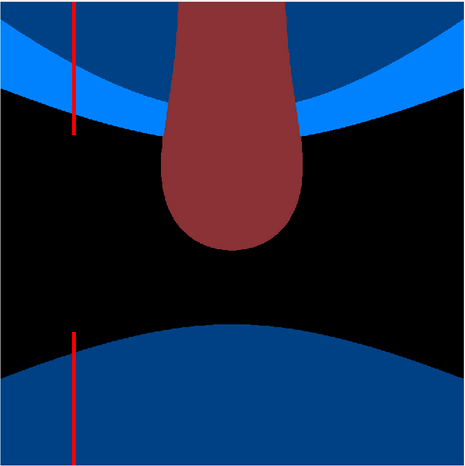
\includegraphics[width=1\linewidth]{Images/2sphere_render.png}
  \captionof{figure}{Generirana slika}
  \label{fig:2sphRend}
\end{minipage}%
\begin{minipage}{.5\textwidth}
  \centering
  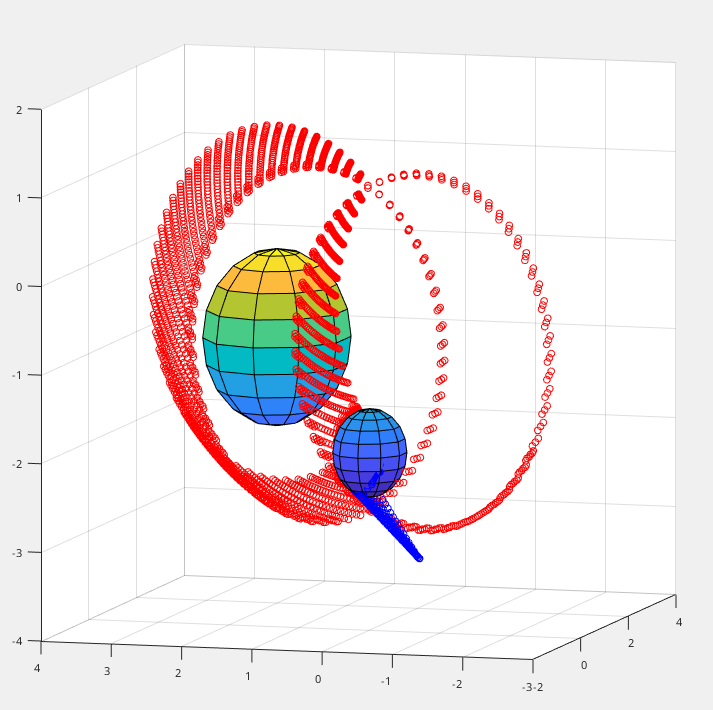
\includegraphics[height=1\linewidth]{Images/2sphere_rays.png}
  \captionof{figure}{Slika snopov žarkov}
  \label{fig:2sphRays}
\end{minipage}
\end{figure}

\bigskip
Če bi spremljali generirane slike ob premikanju kamere, bi videli, da objekti ki so naravnost pred nami pogosto v sliko vstopajo od zgoraj, kar je prav tako pričakovano. Zgornji žarki bodo imeli namreč najdaljši doseg, saj je središče njihove sfere premaknjeno najdlje stran od kamere v smeri premikanja. Na \hyperref[fig:sequence]{sekvenci slik} se mimo rdeče krogle premikamo proti modri krogli, ki je v celoti osvetljena. V ozadju vidimo oranžno ravnino.
\begin{figure}[H]
    \centering
    
\includegraphics[width=1\linewidth]{Images/sequence.png}
    \caption{Zaporedje slik s premikanjem kamere}
    \label{fig:sequence}
\end{figure}
Sceno iz sekvence lahko vidimo na \hyperref[fig:2sphRays2]{sliki žarkov}, kjer je prikazan snop žarkov ene vrstice pikslov.
\begin{figure}[H]
    \centering
    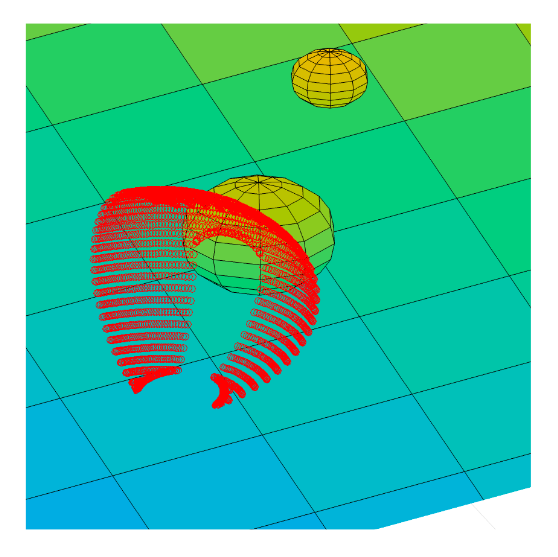
\includegraphics[width=0.4\linewidth]{Images/2sphere_rays2.png}
    \caption{Žarki vrstice pikslov}
    \label{fig:2sphRays2}
\end{figure}


Pomembno je omeniti tudi, da v primeru velikih radijev sfer, po katerih se premikajo žarki, prostor izgleda manj popačeno \ref{fig:2sphere R=25}. 
Slike scene v neevklidskih prosorih vidimo na \ref{fig:Speedup 2sphere scene} in \ref{fig:Speedup euclidean scene}. V prostoru 2sphere, kjer je radij sfere 25, izgleda skoraj kot da bi kamero usmerili v tla. To je 
ponovno posledica dejstva, da objekti pred nami v sliko vstopajo od zgoraj. Opazimo pa tudi, da je krogla na \hyperref[fig:2sphere R=25]{sliki} 
uprizorjena, kot da bi jo gledali z višje točke, kar je posledica ukrivljanja žarkov navzdol.

\begin{figure} [H]
    \centering
    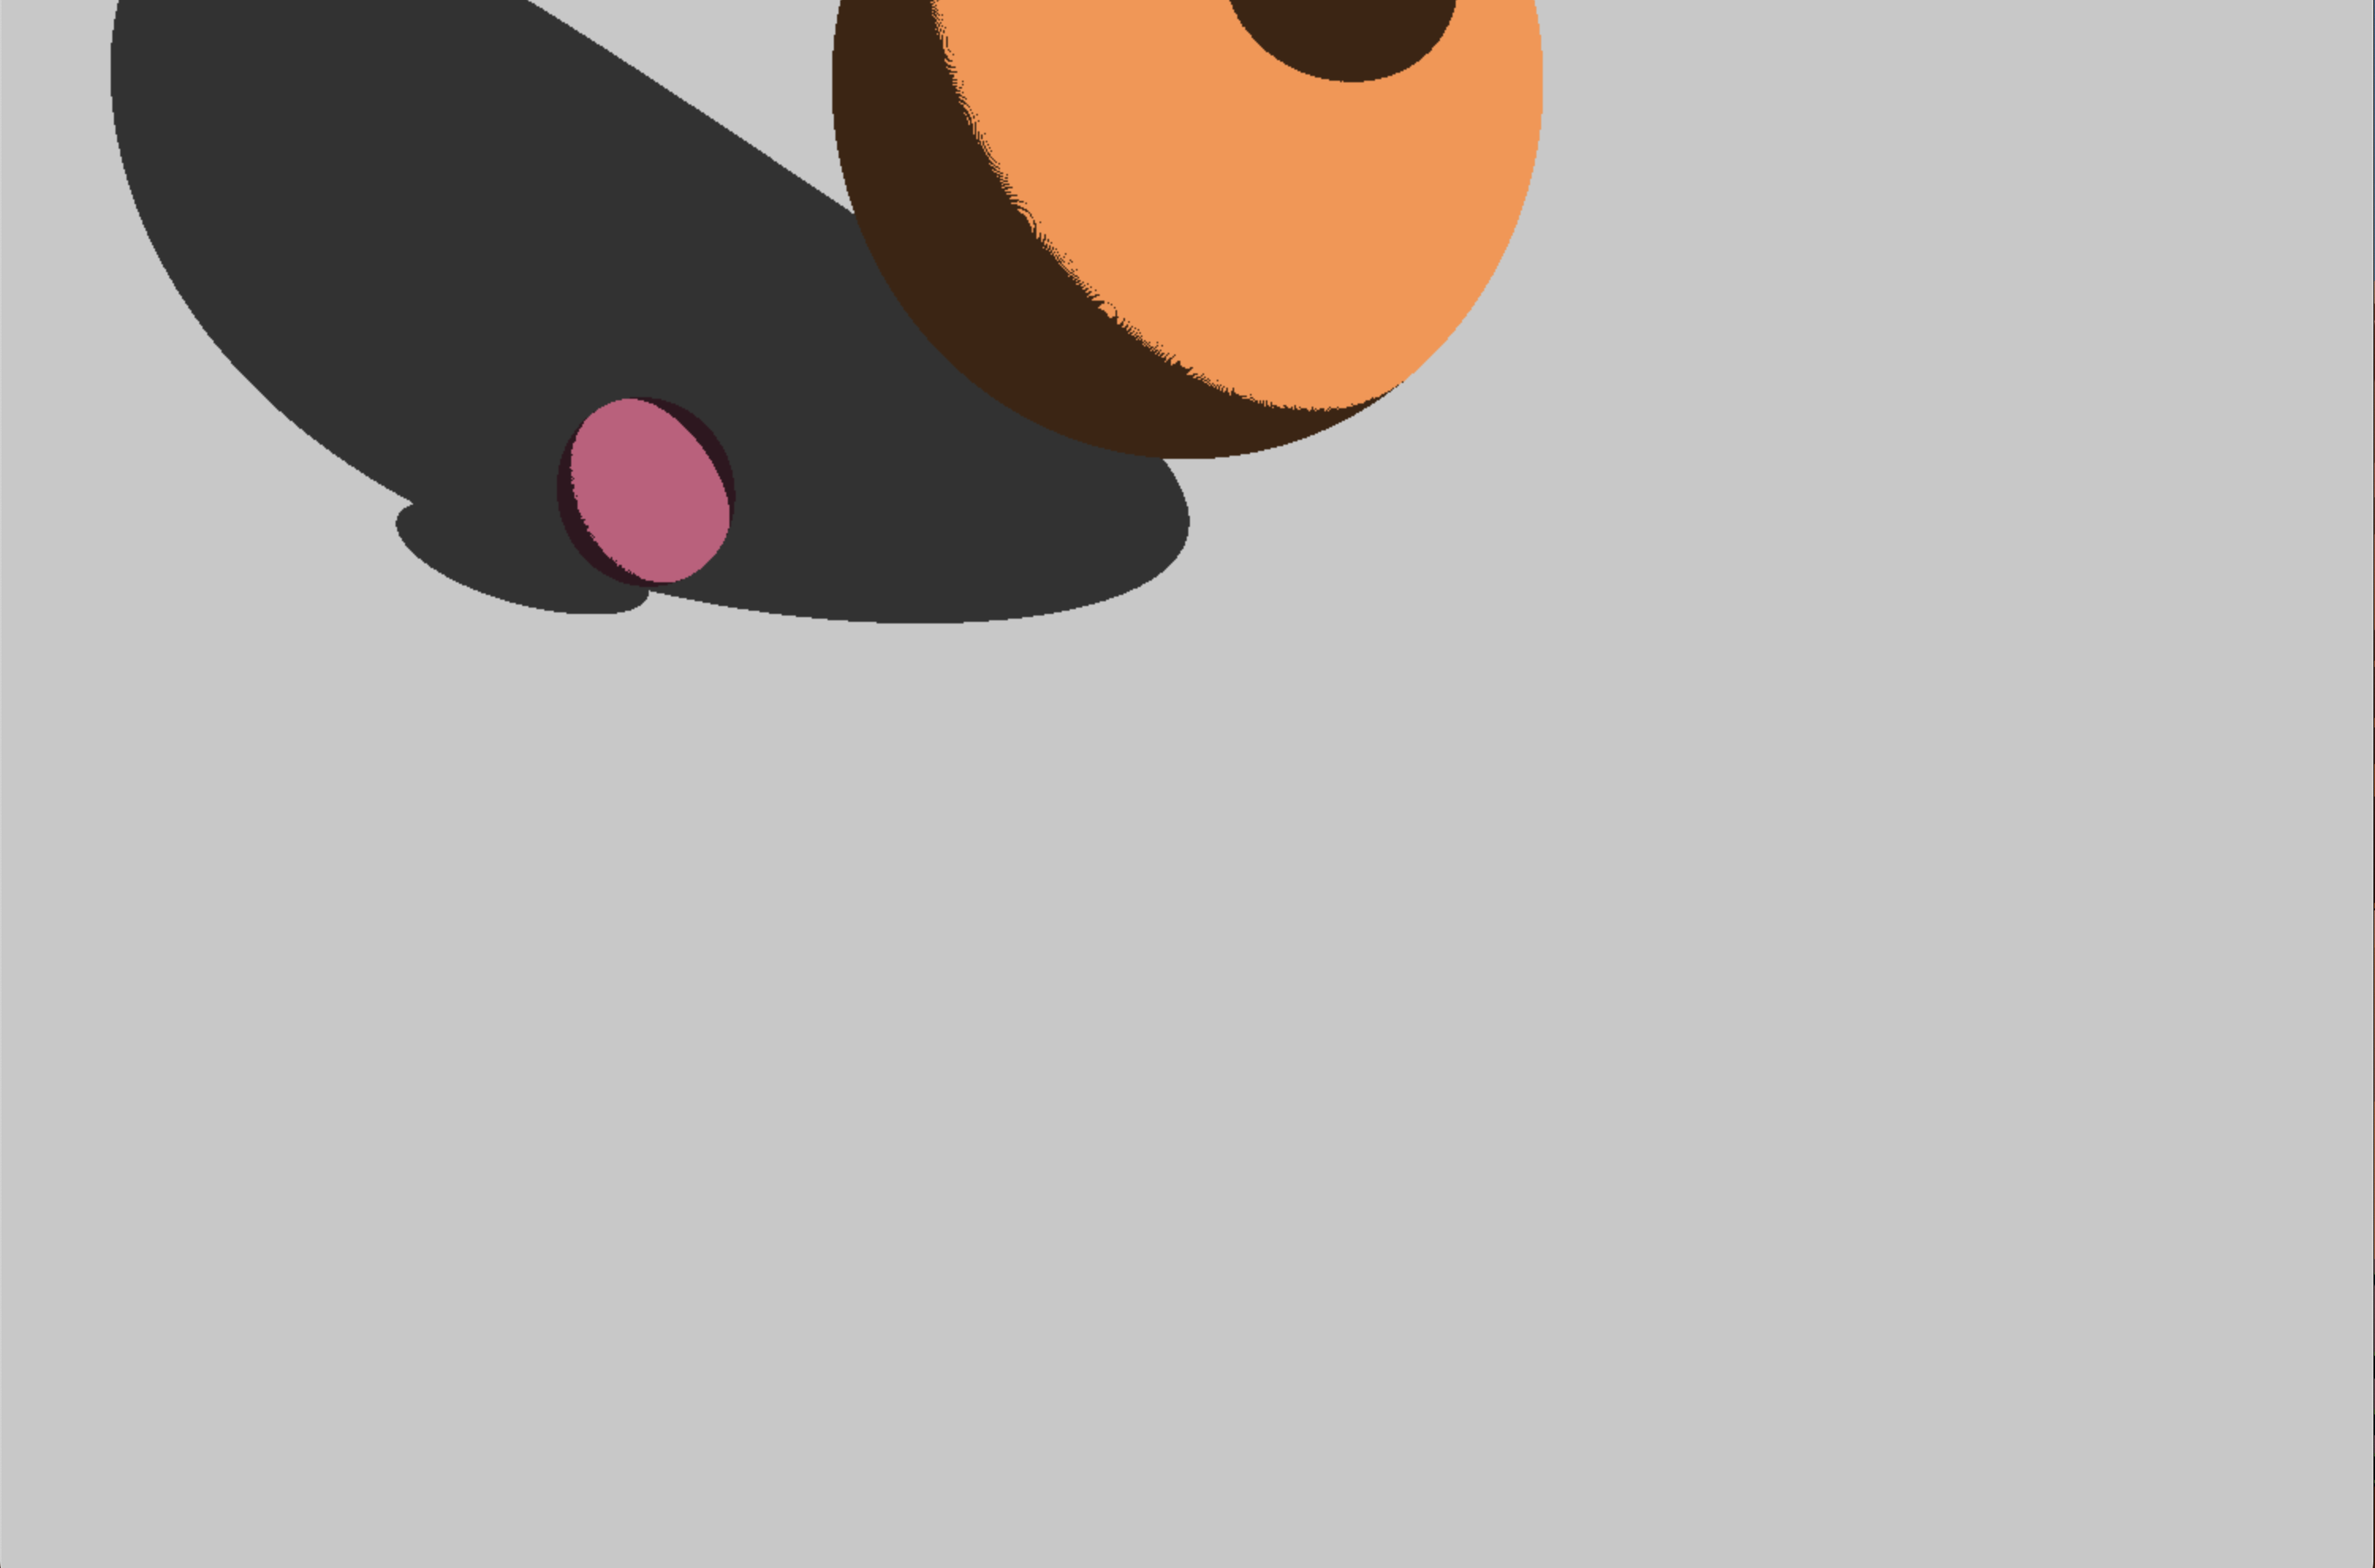
\includegraphics[width=0.6\linewidth]{Images/2sphere_24mm_R=25.png}
    \caption{Render, kjer je radij krogel 25}
    \label{fig:2sphere R=25}
\end{figure}

\section{Primerjava metode sledenje žarku v evklidskem in neevklidskem prostoru}
Primerjamo enako pozicijo kamere in enako postavitev objektov v prostoru v evklidskem in dveh neevklidskih prostorih. Postavitev objektov je enaka kot
na \hyperref[fig:2sphRays2]{sliki žarkov}. Za razliko od evklidskega prostora pri torusu opazimo podvojene objekte, kjer pričakujemo, da bi z večjim številom korakov bilo čedalje manj črnih pikslov. Pri dvodimenzionalni sferi, pri dani postavitvi modre krogle še ne vidimo, rdeča pa je precej popačena. Ploskev pod kroglama je nagnjena, zato pri dvodimenzionalni sferi opazimo, da je spodnji žarki ne zadanejo več.
\begin{figure}[H]
\centering
\begin{minipage}[t]{.33\textwidth}
  \centering
  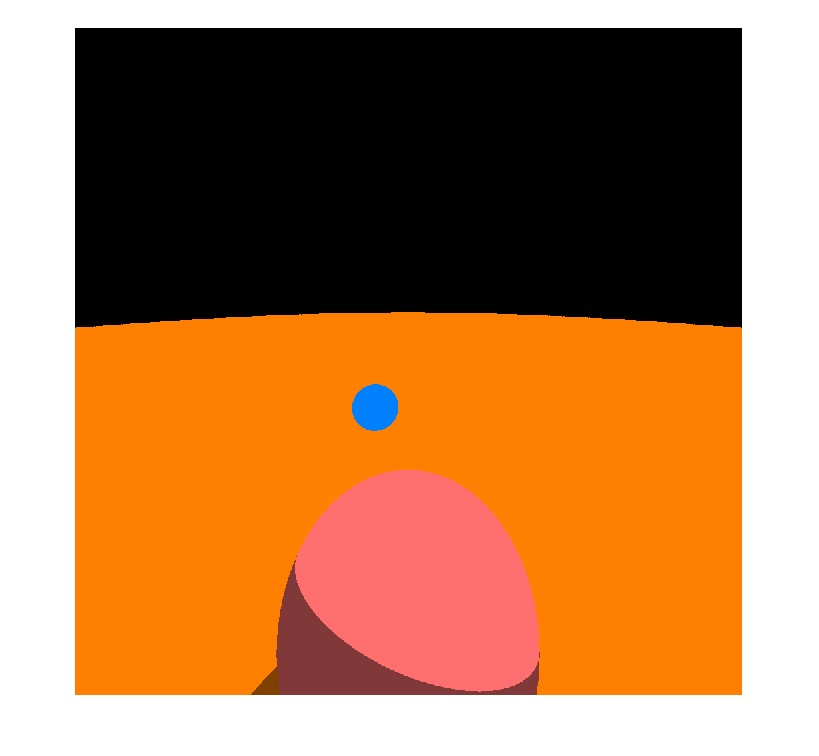
\includegraphics[width=1\linewidth]{Images/Euclidean.jpg}
  \captionof{figure}{Evklidski prostor}
  \label{fig:Evklidski prostor render}
\end{minipage}%
\begin{minipage}[t]{.33\textwidth}
  \centering
  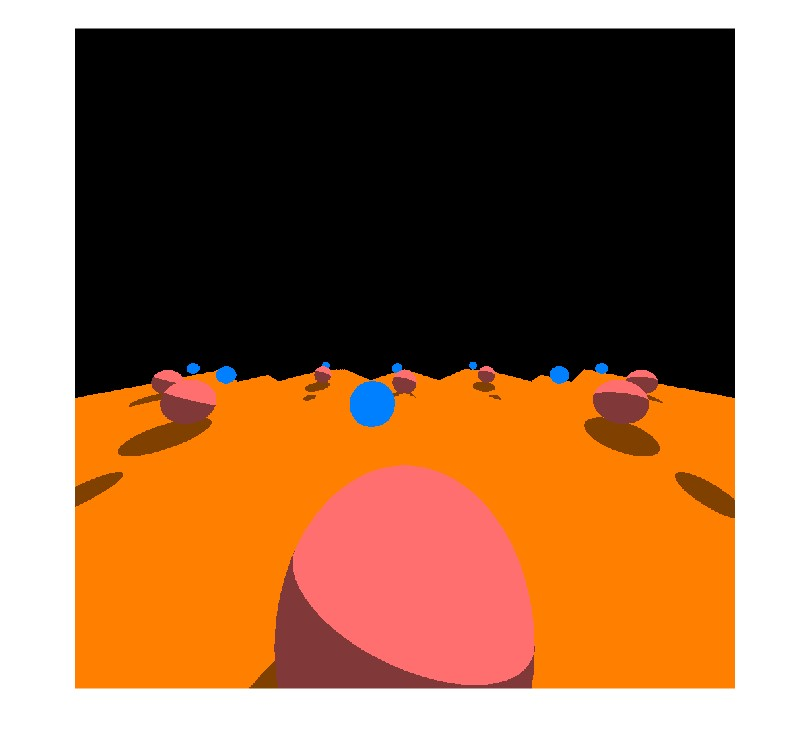
\includegraphics[width=1\linewidth]{Images/Torus.jpg}
  \captionof{figure}{flat torus}
  \label{fig:Flat torus render}
\end{minipage}
\begin{minipage}[t]{.33\textwidth}
  \centering
  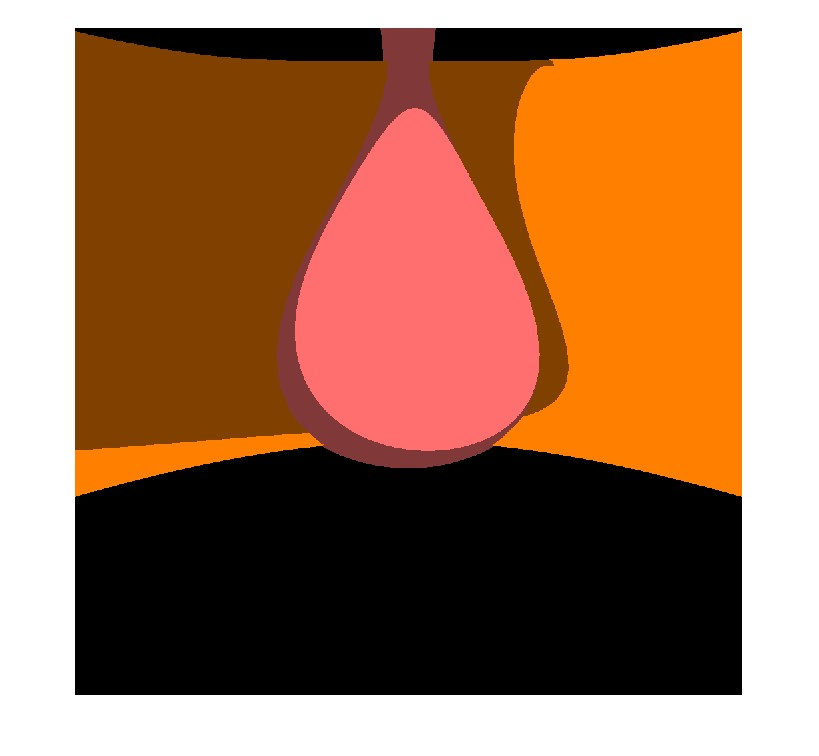
\includegraphics[width=1\linewidth]{Images/2Sphere.jpg}
  \captionof{figure}{Dvodimenzionalna sfera}
  \label{fig:2Sphere render}
\end{minipage}
\end{figure}


\newpage
\section{Pohitritev algoritma}
Da ne bi bilo potrebno na vsako sliko čakati predolgo časa, lahko algoritme pohitrimo. 

\subsection{Pohitritev osnovnega algoritma}
\label{subsec:pohitren_algoritem}
Opazimo naslednji težavi: 
\begin{enumerate}
  \item Korakanje žarka po prostoru hitro postane računsko prezahtevno, če je korak majhen.
  \item Če je korak prevelik, se lahko zgodi, da v neki točki preskoči presečišče z objektom.
\end{enumerate}

\begin{figure} [H]
  \centering
  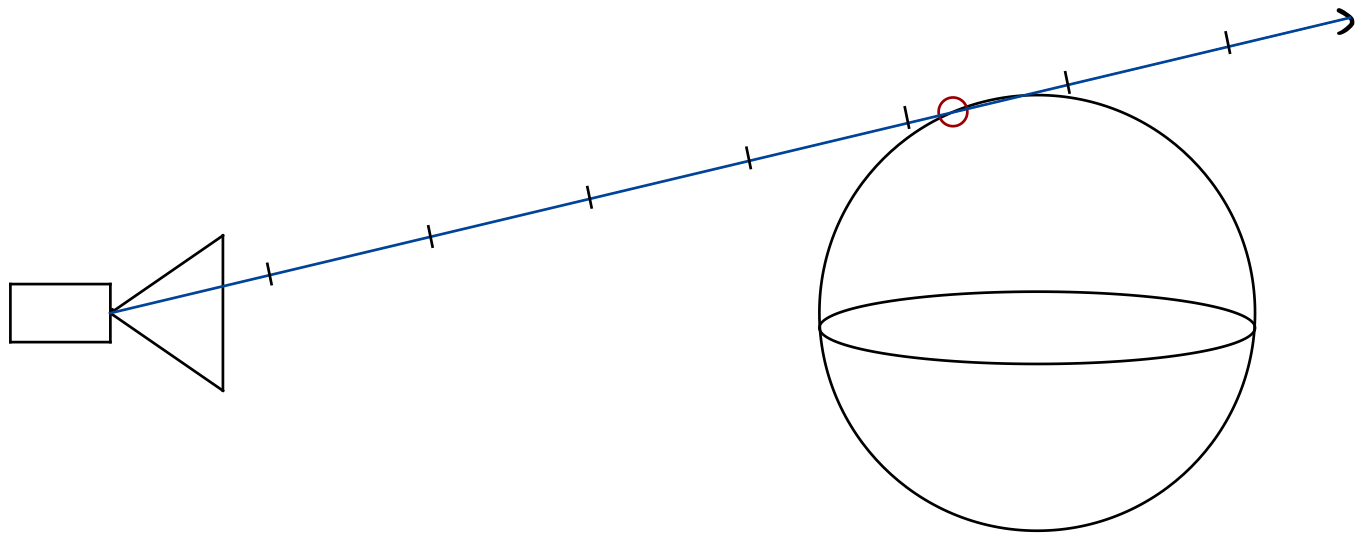
\includegraphics[width=0.6\linewidth]{Images/step_size_issue.png}
  \caption{Zaradi prevelikega koraka, zgrešimo presečišče.}
  \label{fig:step_size_issue}
\end{figure}

Še enkrat se spomnimo, kaj je naš problem. Iščemo najmanjši parameter \( t \), za katerega velja:
\[ f = o(s(t)) = 0 \]
\( o([x, y, z]) = a \) je funkcija (kateregakoli) objekta v sceni, ki je enaka 0 samo, ko je 
točka \([x, y, z]\) na objektu. 
\( s(t, T, \vec{v}) = [x, y, z] \) je funkcija, ki vrne točko v prostoru, kjer se nahaja žarek z izhodiščem v \( T_0\) in smerjo 
\( \vec{v} \) ob času \( t \).


Da bolje razumemo problem, si poglejmo par grafov, ki prikazujejo kako se 
"razdalja" do oranžne krogle (vrednost funkcije \( o(t) \)) spreminja glede na razdaljo žarka od 
kamere (vrednost \( t \)) v evklidskem prostoru in prostoru 2sphere. V sredini slike je obkrožen piksel katerega žarek spremljamo.

\begin{figure}[H]
  \centering
  \begin{minipage}[t]{.4\textwidth}
    \centering
    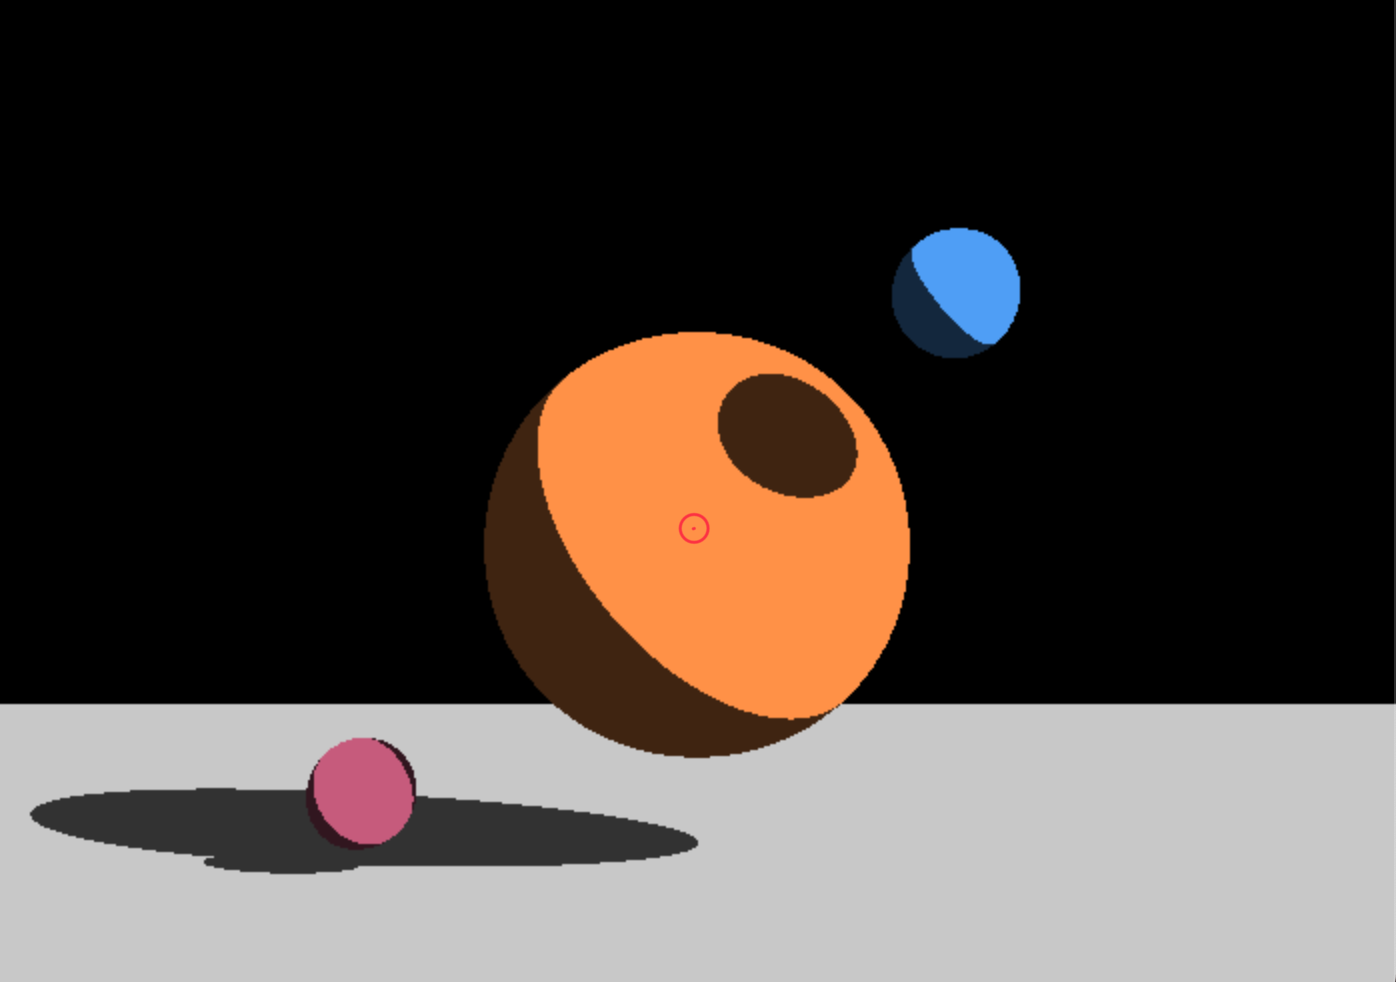
\includegraphics[width=1\linewidth]{Images/speedup_euclidean_scene.png}
    \captionof{figure}{Scena, ki jo bomo pospeševali v evklidskem prostoru}
    \label{fig:Speedup euclidean scene}
  \end{minipage}%
  \hspace{0.04\textwidth} % Added horizontal space
  \begin{minipage}[t]{.4\textwidth}
    \centering
    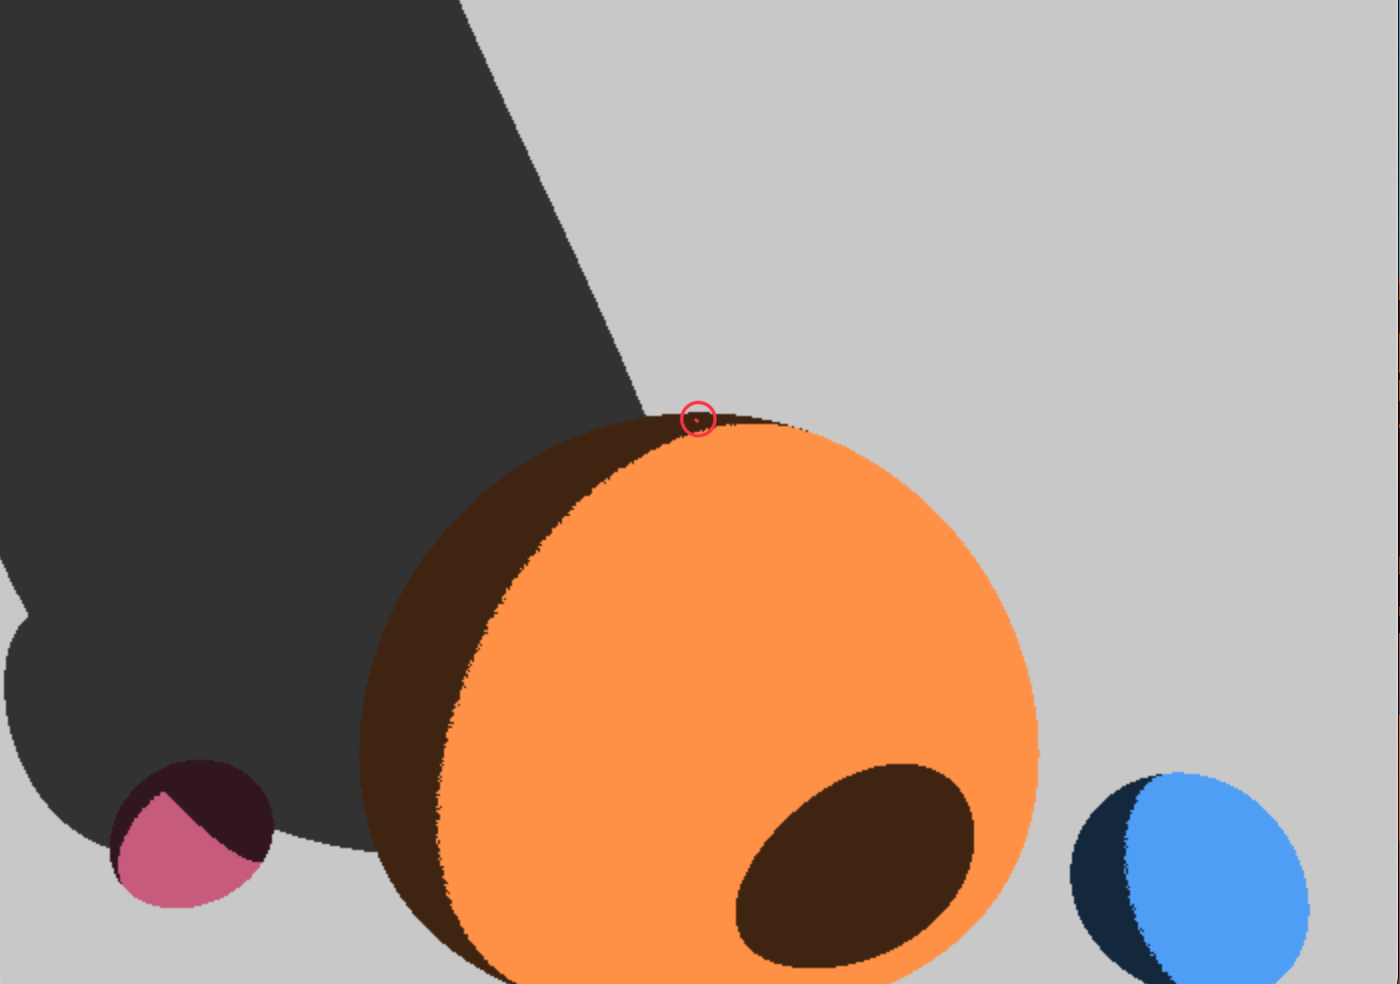
\includegraphics[width=1\linewidth]{Images/speedup_2sphere_scene.png}
    \captionof{figure}{Scena, ki jo bomo pospeševali na 2Sphere}
    \label{fig:Speedup 2sphere scene}
  \end{minipage}
\end{figure}

\begin{figure}[H]
  \centering
  \begin{minipage}[t]{.4\textwidth}
    \centering
    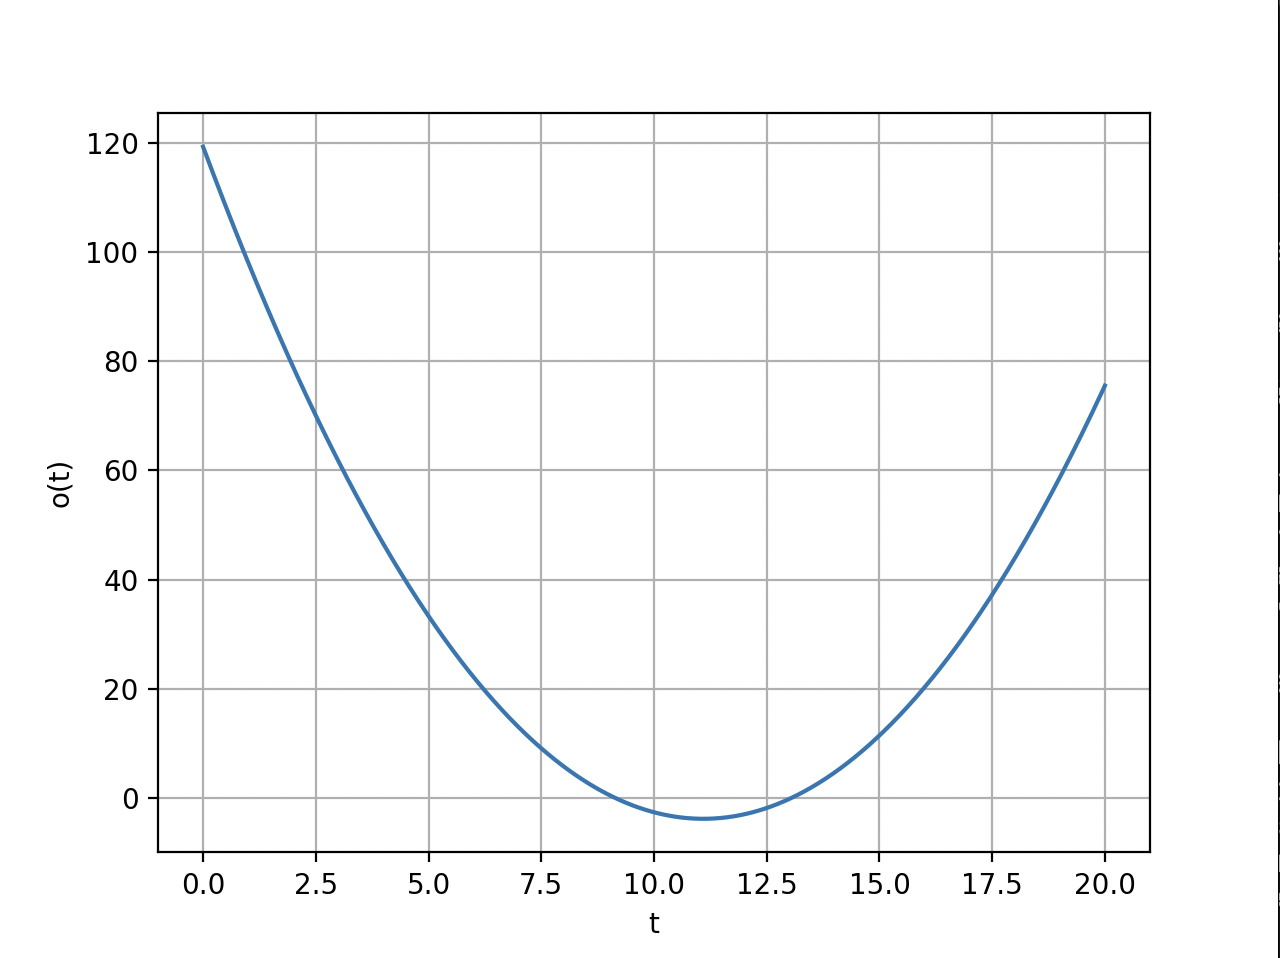
\includegraphics[width=1\linewidth]{Images/speedup_euclidean_graph.png}
    \captionof{figure}{Graf o(t) za evklidski prostor}
    \label{fig:Speedup euclidean graph}
  \end{minipage}%
  \hspace{0.04\textwidth} % Added horizontal space
  \begin{minipage}[t]{.4\textwidth}
    \centering
    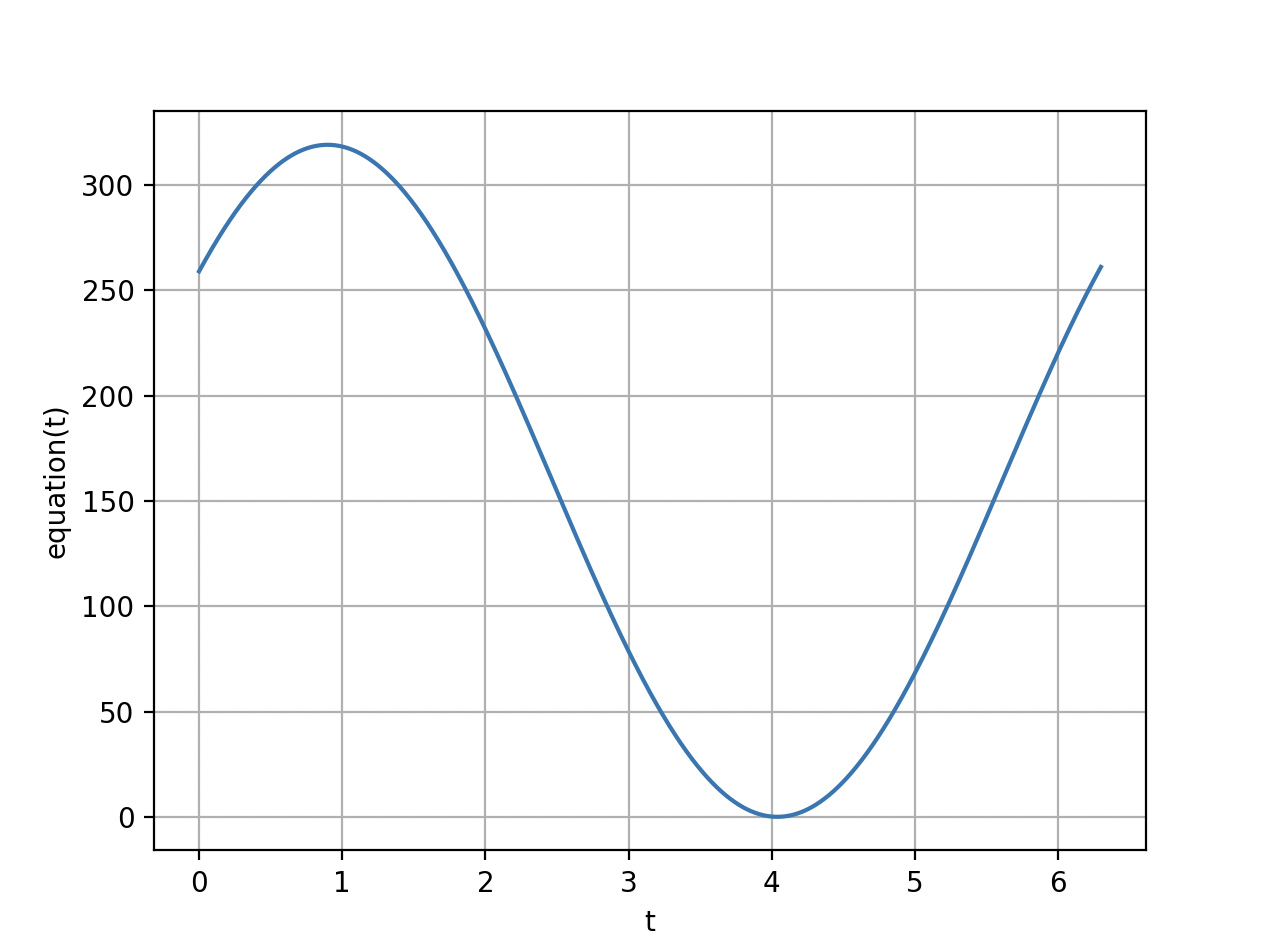
\includegraphics[width=1\linewidth]{Images/speedup_2sphere_graph.png}
    \captionof{figure}{Graf o(t) za 2Sphere}
    \label{fig:Speedup 2sphere graph}
  \end{minipage}
\end{figure}

Hitro nam postane jasno, da razdalja žarka sledi funkciji, ki ima 0, 1, ali 2 ničli (za 2sphere iščemo le na intervalu \(t \in [0, 2\pi] \)). 
Imamo le en minimum za katerega velja, da če je večji od 0, se žarek objekta nikoli ne bo dotaknil.

Implementirali smo naslednje izboljšave osnovnega algoritma:
\begin{itemize}
  \item Ko opazimo, da se funkcija \( o(t) \) začne povečevati, po tem ko je že padala, 
  razpolovimo korak, da preverimo če smo preskočili presečišče
  \item Dokler se funkcija \( o(t) \) ne povečuje, večamo korak, da hitreje pridemo do presečišča.
\end{itemize}

\subsection{Pohitritev iskanja presečišč za euclidean in flat torus}

Ideja je preprosta. Zakaj bi delali iterativne korake, če lahko preprosto izpeljemo 
formulo za izračun parametra \( t \) za katerega velja \( f = 0 \)? Tako presečišče 
najdemo v času odvisnem le od števila objektov v sceni.

Flat torus uporablja kar formulo za presečišče iz evklidskega prostora, le da žarke še preslika, če pridejo do roba torusa.

\subsection{Pohitritev iskanja presečišč za 2Sphere}

Za 2Sphere smo našli rešitev, ki je hitrejša od iterativnega pristopa aproksimacij premikov po geodetkah.

Vsak žarek gre namreč čez vrh in dno sfere. Žarek parametriziramo, kot točko na sferi. Za žarek poiščemo center 
krogle \( [x_0, y_0, z_0] \), kot smo ga prej in za preslikavo na $uv$ ravnino uporabimo enačbi \ref{e:toU} in \ref{e:toV}. 
Parametrizacija žarka \(s(t)\) je torej:

\begin{equation}
  \begin{split}
    &x = R\cos(v)\sin(t) + x_0 \\
    &y = R\sin(v) \sin(t) + y_0 \\
    &z = R\cos(t) + z_0
  \end{split}
\end{equation}

Parametrizacija za razliko od prejšnje ne računa približkov, ampak točno rešitev za katerokoli velikost koraka. 
Zato jo lahko uporabimo v algoritmu\ref{subsec:pohitren_algoritem}.

\section{Zaključek}
Naš cilj je bil narediti program, v katerem se vsak uporabnik lahko igra z različnimi neevklidskimi
prostori in jih vizualizira. To nam je uspelo. Uspelo nam je tudi pospešiti program do te mere, da 
na slike v dokaj visoki resoluciji ni potrebno čakati več kot nekaj deset sekund. Na slike v evklidskem 
prostoru pa, za 1500 x 1000 sliko, celo manj kot 10 sekund.

Sicer obstaja še marsikatera optimizacija in funkcionalnost, ki bi jo lahko dodali,
na primer možnosti dodajanja materialov in boljši algoritem senčenja.

Eden izmed ciljev je bil tudi enostavno dodajanje novih objektov in prostorov:

\begin{figure} [H]
  \centering
  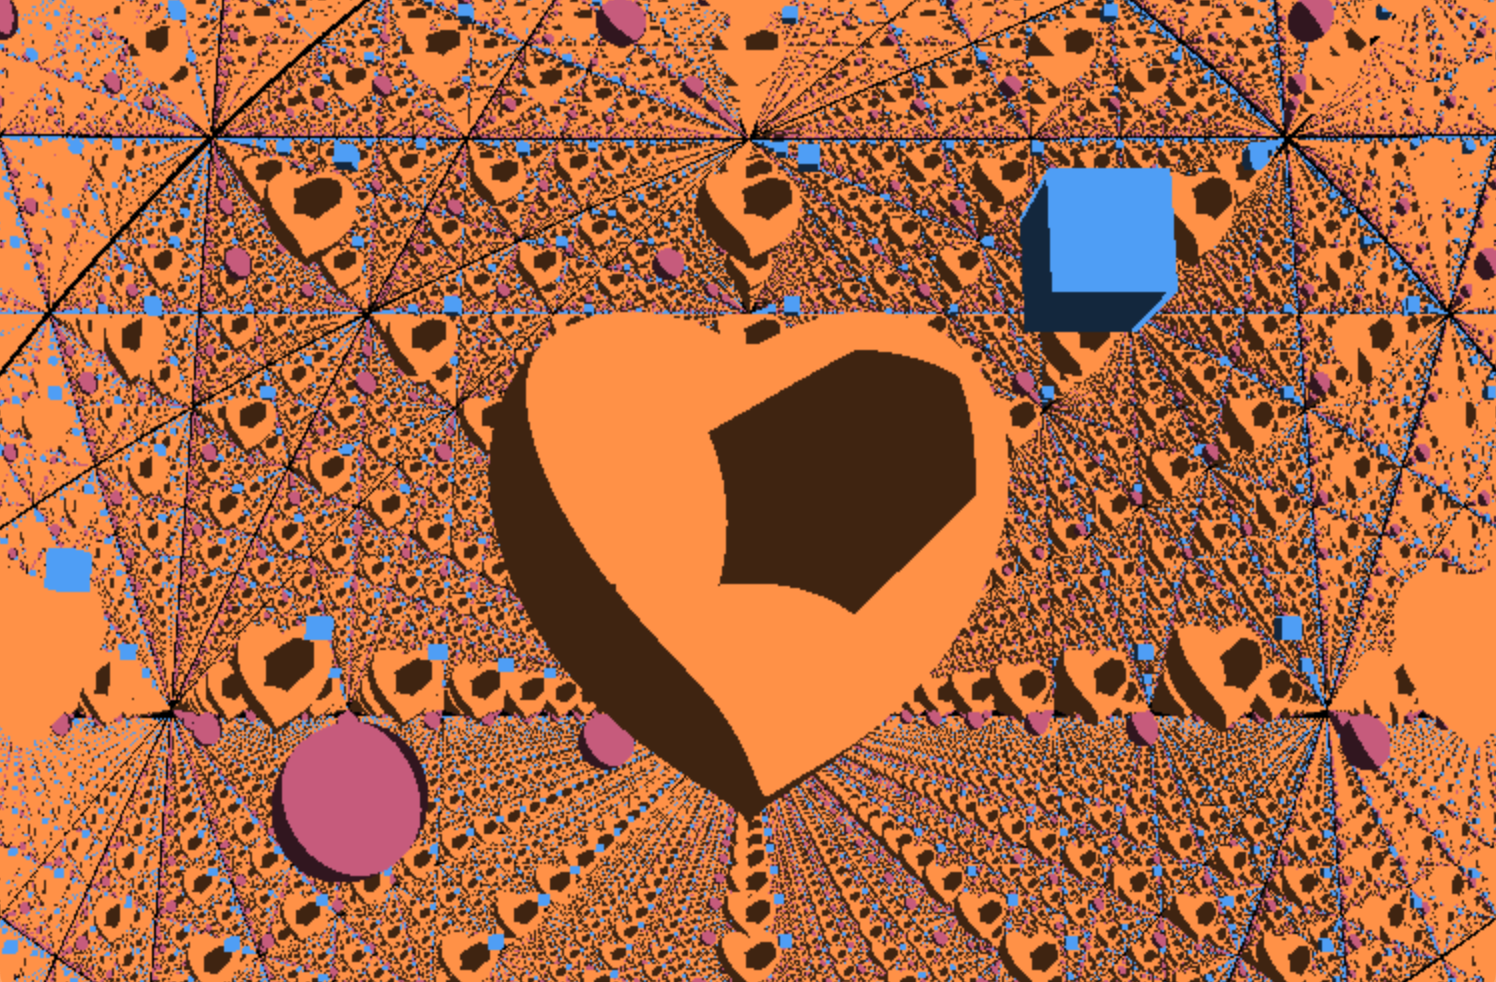
\includegraphics[width=0.9\linewidth]{Images/Flat_torus_24mm_heart_cube.png}
  \caption{Demonstracija dodajanja objektov srca in kocke}
  \label{fig:Flat_torus_heart}
\end{figure}



\section{Razdelitev dela}
\begin{itemize}
  \item Blaž Bergant: Zasnova programa, implementacija osnovnega raytracing algoritma, izpeljava formul za hitrejše delovanje.
  \item Martin Jereb: Priprava poročila, razlaga in implemenacija prostora flat torus, priprava predstavitve.
\item Matjaž Pogačnik: Implementacija in izpeljava algoritmov za 2Sphere, priprava poročila in generiranje slik.
\end{itemize}

\section{Viri}
\begin{itemize}
  \item Kovač, G. (2023). \textit{Sledenje žarku v neevklidskih prostorih} (Diplomska naloga). Ljubljana: [G. Kovač].
  \item Kovač, G. (2024). \textit{Ray tracing in Non-euclidean spaces}. Ljubljana: [G. Kovač].
  \item Zalar, A. \textit{Mathematical Modelling, Lecture Notes} (2024). Ljubljana: [A. Zalar].
  \item \textit{Non-Euclidean geometry}. (2024). Pridobljeno 24.5.2024 s spletne strani: \url{https://en.wikipedia.org/wiki/Non-Euclidean_geometry.}
\end{itemize}

\section{Priloga}
\begin{itemize}
  \item Koda je na voljo na spletnem repozitoriju, na \href{https://github.com/MAZI2/Ray-tracing-non-euclidean-spaces}{povezavi}.
  \item Spletna predstavitev pa je na voljo \href{https://docs.google.com/presentation/d/1NP8gkPzV8rE2ToBoUAP4b7w2yMkAWgCmlsRPMn_5Ahc/edit?usp=sharing}{tukaj}.
\end{itemize}

\end{document}

